\documentclass[ba]{imsart}
%DIF LATEXDIFF DIFFERENCE FILE
%DIF DEL old.tex    Thu Jul 25 15:34:55 2024
%DIF ADD flat.tex   Sun Aug 11 15:11:29 2024
%DIF 2-3d2
%DIF < 
%DIF < % \documentclass[ba,preprint]{imsart}% use this for supplement article
%DIF -------
\usepackage{amsmath}
\usepackage{amssymb}
\usepackage{amsfonts}
\usepackage{amsthm}
%DIF 8c6-8
%DIF < %% \usepackage{amsaddr}
%DIF -------
\usepackage{array}
 %DIF > 
\newcommand*{\vertbar}{\rule[-1ex]{0.5pt}{2.5ex}}
 %DIF > 
\newcommand*{\horzbar}{\rule[.5ex]{2.5ex}{0.5pt}}
 %DIF > 
%DIF -------


%DIF 11-22d11
%DIF < \theoremstyle{plain}
%DIF < \newtheorem{theorem}{Theorem}
%DIF < \newtheorem{corollary}[theorem]{Corollary}
%DIF < \newtheorem{lemma}[theorem]{Lemma}
%DIF < \newtheorem{proposition}[theorem]{Proposition}
%DIF < \theoremstyle{definition}
%DIF < \newtheorem{definition}[theorem]{Definition}
%DIF < \newtheorem{example}[theorem]{Example}
%DIF < \newtheorem{conjecture}[theorem]{Conjecture}
%DIF < \theoremstyle{remark}
%DIF < \newtheorem{remark}[theorem]{Remark}
%DIF < 
%DIF -------
\usepackage{thm-restate}
\usepackage{tikz,pgfplotstable}
\usetikzlibrary{patterns}
%DIF 26-27c14
%DIF < \pgfplotsset{compat=1.9} % set to 1.8 to get old behaviour
%DIF < %\usepackage{hyperref}
%DIF -------
\pgfplotsset{compat=1.9} \usepackage{xcolor}
 %DIF > 
%DIF -------

\newcommand{\R}{\ensuremath{\mathbb{R}}}
\newcommand{\eps}{\varepsilon}
\newcommand{\M}{\mathcal{M}}

\newcommand{\der}{\text{\textup{d}}}
\newcommand{\diag}{\textup{diag}}

\providecommand{\x}{}
\renewcommand{\x}{\mathbf{x}}
\newcommand{\y}{\mathbf{y}}

\newcommand{\hil}{\mathcal{H}}
\newcommand{\hilp}{\mathcal{H}_p}
\newcommand{\hilo}{\mathcal{H}_o}
\newcommand{\obs}{\mathcal{O}}
\newcommand{\pobs}{\mathcal{P}}
\newcommand{\fwd}{\mathcal{F}}

\newcommand{\obsm}{\widehat{\obs}}
\newcommand{\Sigmam}{\widehat{\Sigma}}
\newcommand{\postcovm}{\widehat{\Gamma_{\textup{post}}}}
\newcommand{\uu}{\mathbf{u}}
\newcommand{\tar}{\Psi}
\DeclareMathOperator*{\argmin}{arg\,min}
\DeclareMathOperator*{\argmax}{arg\,max}
%DIF 54a41
\DeclareMathOperator*{\conv}{conv}
 %DIF > 
%DIF -------

%DIF 55c43
%DIF < % Definitions for second chapter
%DIF -------

 %DIF > 
%DIF -------
\newcommand{\data}{\mathbf{d}}
\newcommand{\param}{\mathbf{m}}
\newcommand{\normal}{\mathcal{N}}
%DIF 59-66c47
%DIF < \newcommand{\pr}{\mu_{\textup{pr}}} %Prior measure
%DIF < \newcommand{\post}{\mu_{\textup{post}}^{\data, \obs}} % Posterior measure
%DIF < \newcommand{\prmean}{\param_{\textup{pr}}} % Prior mean
%DIF < \newcommand{\postmean}{\param_{\textup{post}}} % Posterior mean
%DIF < \newcommand{\postcov}{\Gamma_{\textup{post}}} % Posterior covariance
%DIF < \newcommand{\prcov}{\Gamma_{\textup{pr}}} % Prior covariance
%DIF < \newcommand{\modcov}{\Gamma_{\textup{model}}} % Model covariance
%DIF < \newcommand{\tmp}{\mathcal{G}}
%DIF -------
\newcommand{\pr}{\mu_{\textup{pr}}} \newcommand{\post}{\mu_{\textup{post}}} \newcommand{\prmean}{\param_{\textup{pr}}} \newcommand{\postmean}{\param_{\textup{post}}} \newcommand{\postcov}{\Gamma_{\textup{post}}} \newcommand{\prcov}{\Gamma_{\textup{pr}}} \newcommand{\modcov}{\Gamma_{\textup{model}}} \newcommand{\tmp}{\mathcal{G}}
 %DIF > 
%DIF -------
\newcommand{\meas}{\mathbf{o}}
%DIF 68-69c49
%DIF < \newcommand{\ev}{\mathbf{e}} % eigenvector 
%DIF < \newcommand{\func}{\mathbf{a}}
%DIF -------
\newcommand{\ev}{\mathbf{e}} \newcommand{\func}{\mathbf{a}}
 %DIF > 
%DIF -------
\newcommand{\tr}[1]{\textup{tr}\left \{#1 \right \} }
\newcommand{\ttr}[1]{\textup{tr}\ #1}
\newcommand{\rank}{\textup{rank}\ }
%DIF 73-74c53
%DIF < \newcommand{\des}{\eta} % vector of design parameters
%DIF < \newcommand{\sigsqr}{\sigma^2}
%DIF -------
\newcommand{\des}{\eta} \newcommand{\sigsqr}{\sigma^2}
 %DIF > 
%DIF -------

%DIF 76a55-56
\newcommand{\opt}{\mathcal{D}}
 %DIF > 
\newcommand{\postopt}{\mu_{\textup{post}}^{\data, \opt}} 
 %DIF > 
%DIF -------

%DIF 77-80d58
%DIF < %% %\usepackage{comment}% http://ctan.org/pkg/comment
%DIF < %% %% %% %\excludecomment{proof}
%DIF < %% %% \excludecomment{figure}
%DIF < %% %% \let\endfigure\relax
%DIF -------


%DIF 83c60-70
%DIF < %% %\overfullrule=0pt
%DIF -------
\theoremstyle{plain}
 %DIF > 
\newtheorem{theorem}{Theorem}
 %DIF > 
\newtheorem{corollary}[theorem]{Corollary}
 %DIF > 
\newtheorem{lemma}[theorem]{Lemma}
 %DIF > 
\newtheorem{proposition}[theorem]{Proposition}
 %DIF > 
\theoremstyle{definition}
 %DIF > 
\newtheorem{definition}[theorem]{Definition}
 %DIF > 
\newtheorem{example}[theorem]{Example}
 %DIF > 
\newtheorem{conjecture}[theorem]{Conjecture}
 %DIF > 
\theoremstyle{remark}
 %DIF > 
\newtheorem{remark}[theorem]{Remark}
 %DIF > 
%DIF -------
 
%DIF 85d72
%DIF < %
%DIF -------
\pubyear{2021}
\volume{TBA}
\issue{TBA}
%DIF 89-90d75
%DIF < % \doi{0000}
%DIF < %\arxiv{}
%DIF -------
\firstpage{1}
\lastpage{1}

\usepackage{amsthm}
\usepackage{amsmath}
\usepackage{natbib}
\usepackage[colorlinks,citecolor=blue,urlcolor=blue,filecolor=blue,backref=page]{hyperref}
\usepackage{graphicx}

\startlocaldefs
%DIF 101d85
%DIF < % ** Local definitions **
%DIF -------
\endlocaldefs
%DIF PREAMBLE EXTENSION ADDED BY LATEXDIFF
%DIF UNDERLINE PREAMBLE %DIF PREAMBLE
\RequirePackage[normalem]{ulem} %DIF PREAMBLE
\RequirePackage{color}\definecolor{RED}{rgb}{1,0,0}\definecolor{BLUE}{rgb}{0,0,1} %DIF PREAMBLE
\providecommand{\DIFaddtex}[1]{{\protect\color{blue}\uwave{#1}}} %DIF PREAMBLE
\providecommand{\DIFdeltex}[1]{{\protect\color{red}\sout{#1}}}                      %DIF PREAMBLE
%DIF SAFE PREAMBLE %DIF PREAMBLE
\providecommand{\DIFaddbegin}{} %DIF PREAMBLE
\providecommand{\DIFaddend}{} %DIF PREAMBLE
\providecommand{\DIFdelbegin}{} %DIF PREAMBLE
\providecommand{\DIFdelend}{} %DIF PREAMBLE
\providecommand{\DIFmodbegin}{} %DIF PREAMBLE
\providecommand{\DIFmodend}{} %DIF PREAMBLE
%DIF FLOATSAFE PREAMBLE %DIF PREAMBLE
\providecommand{\DIFaddFL}[1]{\DIFadd{#1}} %DIF PREAMBLE
\providecommand{\DIFdelFL}[1]{\DIFdel{#1}} %DIF PREAMBLE
\providecommand{\DIFaddbeginFL}{} %DIF PREAMBLE
\providecommand{\DIFaddendFL}{} %DIF PREAMBLE
\providecommand{\DIFdelbeginFL}{} %DIF PREAMBLE
\providecommand{\DIFdelendFL}{} %DIF PREAMBLE
%DIF HYPERREF PREAMBLE %DIF PREAMBLE
\providecommand{\DIFadd}[1]{\texorpdfstring{\DIFaddtex{#1}}{#1}} %DIF PREAMBLE
\providecommand{\DIFdel}[1]{\texorpdfstring{\DIFdeltex{#1}}{}} %DIF PREAMBLE
\newcommand{\DIFscaledelfig}{0.5}
%DIF HIGHLIGHTGRAPHICS PREAMBLE %DIF PREAMBLE
\RequirePackage{settobox} %DIF PREAMBLE
\RequirePackage{letltxmacro} %DIF PREAMBLE
\newsavebox{\DIFdelgraphicsbox} %DIF PREAMBLE
\newlength{\DIFdelgraphicswidth} %DIF PREAMBLE
\newlength{\DIFdelgraphicsheight} %DIF PREAMBLE
% store original definition of \includegraphics %DIF PREAMBLE
\LetLtxMacro{\DIFOincludegraphics}{\includegraphics} %DIF PREAMBLE
\newcommand{\DIFaddincludegraphics}[2][]{{\color{blue}\fbox{\DIFOincludegraphics[#1]{#2}}}} %DIF PREAMBLE
\newcommand{\DIFdelincludegraphics}[2][]{% %DIF PREAMBLE
\sbox{\DIFdelgraphicsbox}{\DIFOincludegraphics[#1]{#2}}% %DIF PREAMBLE
\settoboxwidth{\DIFdelgraphicswidth}{\DIFdelgraphicsbox} %DIF PREAMBLE
\settoboxtotalheight{\DIFdelgraphicsheight}{\DIFdelgraphicsbox} %DIF PREAMBLE
\scalebox{\DIFscaledelfig}{% %DIF PREAMBLE
\parbox[b]{\DIFdelgraphicswidth}{\usebox{\DIFdelgraphicsbox}\\[-\baselineskip] \rule{\DIFdelgraphicswidth}{0em}}\llap{\resizebox{\DIFdelgraphicswidth}{\DIFdelgraphicsheight}{% %DIF PREAMBLE
\setlength{\unitlength}{\DIFdelgraphicswidth}% %DIF PREAMBLE
\begin{picture}(1,1)% %DIF PREAMBLE
\thicklines\linethickness{2pt} %DIF PREAMBLE
{\color[rgb]{1,0,0}\put(0,0){\framebox(1,1){}}}% %DIF PREAMBLE
{\color[rgb]{1,0,0}\put(0,0){\line( 1,1){1}}}% %DIF PREAMBLE
{\color[rgb]{1,0,0}\put(0,1){\line(1,-1){1}}}% %DIF PREAMBLE
\end{picture}% %DIF PREAMBLE
}\hspace*{3pt}}} %DIF PREAMBLE
} %DIF PREAMBLE
\LetLtxMacro{\DIFOaddbegin}{\DIFaddbegin} %DIF PREAMBLE
\LetLtxMacro{\DIFOaddend}{\DIFaddend} %DIF PREAMBLE
\LetLtxMacro{\DIFOdelbegin}{\DIFdelbegin} %DIF PREAMBLE
\LetLtxMacro{\DIFOdelend}{\DIFdelend} %DIF PREAMBLE
\DeclareRobustCommand{\DIFaddbegin}{\DIFOaddbegin \let\includegraphics\DIFaddincludegraphics} %DIF PREAMBLE
\DeclareRobustCommand{\DIFaddend}{\DIFOaddend \let\includegraphics\DIFOincludegraphics} %DIF PREAMBLE
\DeclareRobustCommand{\DIFdelbegin}{\DIFOdelbegin \let\includegraphics\DIFdelincludegraphics} %DIF PREAMBLE
\DeclareRobustCommand{\DIFdelend}{\DIFOaddend \let\includegraphics\DIFOincludegraphics} %DIF PREAMBLE
\LetLtxMacro{\DIFOaddbeginFL}{\DIFaddbeginFL} %DIF PREAMBLE
\LetLtxMacro{\DIFOaddendFL}{\DIFaddendFL} %DIF PREAMBLE
\LetLtxMacro{\DIFOdelbeginFL}{\DIFdelbeginFL} %DIF PREAMBLE
\LetLtxMacro{\DIFOdelendFL}{\DIFdelendFL} %DIF PREAMBLE
\DeclareRobustCommand{\DIFaddbeginFL}{\DIFOaddbeginFL \let\includegraphics\DIFaddincludegraphics} %DIF PREAMBLE
\DeclareRobustCommand{\DIFaddendFL}{\DIFOaddendFL \let\includegraphics\DIFOincludegraphics} %DIF PREAMBLE
\DeclareRobustCommand{\DIFdelbeginFL}{\DIFOdelbeginFL \let\includegraphics\DIFdelincludegraphics} %DIF PREAMBLE
\DeclareRobustCommand{\DIFdelendFL}{\DIFOaddendFL \let\includegraphics\DIFOincludegraphics} %DIF PREAMBLE
%DIF COLORLISTINGS PREAMBLE %DIF PREAMBLE
\RequirePackage{listings} %DIF PREAMBLE
\RequirePackage{color} %DIF PREAMBLE
\lstdefinelanguage{DIFcode}{ %DIF PREAMBLE
%DIF DIFCODE_UNDERLINE %DIF PREAMBLE
  moredelim=[il][\color{red}\sout]{\%DIF\ <\ }, %DIF PREAMBLE
  moredelim=[il][\color{blue}\uwave]{\%DIF\ >\ } %DIF PREAMBLE
} %DIF PREAMBLE
\lstdefinestyle{DIFverbatimstyle}{ %DIF PREAMBLE
	language=DIFcode, %DIF PREAMBLE
	basicstyle=\ttfamily, %DIF PREAMBLE
	columns=fullflexible, %DIF PREAMBLE
	keepspaces=true %DIF PREAMBLE
} %DIF PREAMBLE
\lstnewenvironment{DIFverbatim}{\lstset{style=DIFverbatimstyle}}{} %DIF PREAMBLE
\lstnewenvironment{DIFverbatim*}{\lstset{style=DIFverbatimstyle,showspaces=true}}{} %DIF PREAMBLE
%DIF END PREAMBLE EXTENSION ADDED BY LATEXDIFF

\begin{document}



%DIF < % *** Frontmatter *** 
\DIFdelbegin %DIFDELCMD < 

%DIFDELCMD < %%%
\DIFdelend \begin{frontmatter}
\title{Measurement Clusterization in Bayesian D-optimal Designs in Infinite Dimensions}

%DIF < \title{\support{}}
\runtitle{Measurement Clusterization in D-optimal Designs}
%DIF < \author{Yair Daon}
%DIF < \numberwithin{equation}{section}


\begin{aug}
\author{\fnms{Yair} \snm{Daon}\thanksref{addr1}\ead[label=e1]{yair.daon@gmail.com}}
\runauthor{Yair Daon}

\DIFdelbegin %DIFDELCMD < \address[addr1]{Azrieli Faculty of Medicine, Bar-Ilan University, Safed, Israel
%DIFDELCMD <     \printead{e1} % print email address of "e1"
%DIFDELCMD < }
%DIFDELCMD < %%%
\DIFdelend \DIFaddbegin \address[addr1]{Azrieli Faculty of Medicine, Bar-Ilan University, Safed, Israel
    \printead{e1} }
\DIFaddend 

\end{aug}

\begin{abstract}
  Estimation of parameters in physical processes often demands costly measurements, prompting the pursuit of an optimal measurement strategy. Finding such strategy is termed the problem of \emph{optimal experimental design}, abbreviated as optimal design. Remarkably, optimal designs can yield tightly clustered measurement locations, leading researchers to fundamentally revise the design problem just to circumvent this issue. Some authors introduce error correlation among error terms that are initially independent, while others restrict measurement locations to a finite set of locations. While both approaches may prevent clusterization, they also fundamentally alter the optimal design problem.

In this study, we consider Bayesian D-optimal designs, i.e.~designs that maximize the expected Kullback-Leibler divergence between posterior and prior. We propose an analytically tractable model for D-optimal designs over Hilbert spaces. In this framework, we make several key contributions: \textbf{(a)} We establish that measurement clusterization is a generic trait of D-optimal designs with independent Gaussian measurement errors, and prove that introducing correlations among measurement error terms mitigates clusterization. \textbf{(b)} We characterize D-optimal designs as reducing uncertainty across a subset of prior covariance eigenvectors. Finally, \textbf{(c)} We leverage this characterization to argue that measurement clusterization arises as a consequence of the pigeonhole principle: when more measurements are taken than there are locations where the select eigenvectors are large and others are small --- clusterization occurs. 
 %DIF < 
%DIF < % In summary, in this study we shed light on an often ignored issue with
%DIF < % Bayesian D-optimal designs. We characterize such designs and show why
%DIF < % clusterization arisesit arisestheir inherent properties, propose
%DIF < % strategies to address clusterization, and provide insights into the
%DIF < % fundamental attributes underlying measurement design optimization.
\end{abstract}

%DIF < % ** Keywords **
\begin{keyword}[class=MSC]
\kwd[Primary ]{62F15}
\kwd{35R30}
\kwd[; secondary ]{28C20}
\end{keyword}

\end{frontmatter}

\section{Introduction}\label{section:intro}
\DIFdelbegin \DIFdel{Measurements play a fundamental role in generating observations and are indispensable to any inference process.
Selecting the optimal }\DIFdelend \DIFaddbegin \DIFadd{The practice of experimental design entails specifying every detail of
running an experiment \mbox{%DIFAUXCMD
\cite{chaloner1995}}\hskip0pt%DIFAUXCMD
. At its simplest form,
experimental design involves choosing a set of measurements to be
taken. For example, consider the process of searching for oil:
measurements require digging holes in the ground and a }\emph{\DIFadd{design}}
\DIFadd{simply indicates which holes should be dug
\mbox{%DIFAUXCMD
\cite{horesh2008borehole}}\hskip0pt%DIFAUXCMD
. Since measurements are expensive, only a
limited number of them can be taken, and thus carefully choosing
measurement locations is crucial.
}

\DIFadd{Specifying the right }\DIFaddend set of measurements holds particular significance
when \DIFdelbegin \DIFdel{inferring
parameters of
a physical process. Unlike many other fields, where
measurements are fixed, in this context, we have the freedom to choose
which measurements to take. This freedom should be taken advantage of :
measurements should be chosen to enhance accuracy, reduce costs, or
both. Whether measurements involve specifying }\DIFdelend \DIFaddbegin \DIFadd{solving an }\emph{\DIFadd{inverse problem}} \DIFadd{--- i.e.~making inference of
the physical world utilizing a physical model of a phenomenon of
interest \mbox{%DIFAUXCMD
\cite{tarantola2005,kaipio2005}}\hskip0pt%DIFAUXCMD
. In an inverse problem, we
seek to infer physical quantities, based on observations and a model
of the physical world. Models are typically phrased in the language of
ordinary or partial differential equations.
}

\DIFadd{Inverse problems are ubiquitous in science and engineering. For
example, in electrical impedance tomography (EIT) we seek to infer the
structure of the inside of a human body. Inference is conducted based
on observations of electrical current impedance measured at specific
}\DIFaddend electrode locations on the skin\DIFdelbegin \DIFdel{in electric impedance tomography \mbox{%DIFAUXCMD
\cite{horesh2010impedance}}\hskip0pt%DIFAUXCMD
,
determining certain wavelengths in MRI \mbox{%DIFAUXCMD
\cite{horesh2008mri}}\hskip0pt%DIFAUXCMD
,
positioning sensors for detecting ground-reflected waves in the search
for oil \mbox{%DIFAUXCMD
\cite{horesh2008borehole}}\hskip0pt%DIFAUXCMD
, or optimizing sensor locations in a seismographic network \mbox{%DIFAUXCMD
\cite{rabinowitz1990, steinberg1995}
}\hskip0pt%DIFAUXCMD
--- the
selection of
optimal measurements , referred to as the problem of
}\emph{\DIFdel{optimal design}}%DIFAUXCMD
\DIFdel{, becomes crucial. Optimal measurements are
chosen according to
specific }\emph{\DIFdel{design criteria}}%DIFAUXCMD
\DIFdel{, with A- and D-optimality being two }\DIFdelend \DIFaddbegin \DIFadd{, leveraging known equations of
electric current flow \mbox{%DIFAUXCMD
\cite{horesh2010impedance}}\hskip0pt%DIFAUXCMD
. Magnetic Resonance
Imaging (MRI) also entails solving an inverse problem. There,
radio-frequency pulses are sent through the human body in the presence
of a strong magnetic field. The response of one's body contents to
these radio-frequency pulses is measured, allowing a radiologist to
view the internals of a body in a noninvasive manner
\mbox{%DIFAUXCMD
\cite{horesh2008mri}}\hskip0pt%DIFAUXCMD
. An inverse problem also arises in oil and gas
exploration, where acoustic waves are sent through "boreholes" ---
deep cylindrical wells drilled into the ground. Data of travel and
return times of the acoustic waves are recorded. Wave travel and
return time is influenced by the properties of the subsurface
materials, such as density, elasticity, and the presence of fluids or
voids. Combining travel time data with a geophysical models of
contents of the earth's crust facilitates reconstructing the structure
of the subsurface in a process called }\emph{\DIFadd{borehole tomography}}
\DIFadd{\mbox{%DIFAUXCMD
\cite{horesh2008borehole}}\hskip0pt%DIFAUXCMD
. Inverse problems also arise in many other
areas of seismology and geology \mbox{%DIFAUXCMD
\cite{rabinowitz1990, steinberg1995}
}\hskip0pt%DIFAUXCMD
and medical imaging \mbox{%DIFAUXCMD
\cite{tarantola2005}}\hskip0pt%DIFAUXCMD
. In many inverse problems the
goal is to infer some numerical parameter. However, in the formulation
we consider in this study, as well as in the examples above, the goal
is to conduct inference over some }\emph{\DIFadd{function}} \DIFadd{over $\Omega$, where
\(\Omega \subseteq \mathbb{R}^d, d=1,2,3\) is a spatial domain of
interest.
}

\subsection{\DIFadd{D-optimal Designs}}\label{subsec:D}
\DIFadd{In all of the examples of inverse problems we have seen, as well as in
many other applications, only a limited number of measurements are
allowed. For example, in borehole tomography, a measurement involves
drilling a deep well in the ground --- a very costly endeavor. Even in
a seemingly simpler application such as MRI, a patient cannot occupy
the MRI machine for too long, hence only a limited number of
measurements can be taken. Therefore, measurements should be chosen to
most benefit the user. Typically, a user will consider some utility,
called a }\emph{\DIFadd{design criterion}} \DIFadd{and take measurements that maximize
this utility. Two }\DIFaddend of the most widely recognized and extensively
studied design criteria \DIFdelbegin \DIFdel{\mbox{%DIFAUXCMD
\cite{Chaloner1995,
  AlexanderianGloorGhattas14}}\hskip0pt%DIFAUXCMD
}\DIFdelend \DIFaddbegin \DIFadd{are the A- and }\emph{\DIFadd{D-optimality}} \DIFadd{criteria}\DIFaddend .

\DIFdelbegin \DIFdel{Surprisingly, A- and }\DIFdelend \DIFaddbegin \DIFadd{In this study, we focus on the Bayesian D-optimality
criterion. Bayesian D-optimality carries a simple and intuitive
meaning: measurements chosen according to the D-optimality criterion
maximize the expected Kullback-Leibler (KL) divergence from posterior
to prior \mbox{%DIFAUXCMD
\cite{chaloner1995, AlexanderianGloorGhattas14,
  CoverThomas91}}\hskip0pt%DIFAUXCMD
. Utilizing KL divergence for quantifying differences
between distributions is standard practice and we will not motivate it
further here. For a discrete parameter $\param$ and data $\data$, the
KL divergence is defined as
}\begin{equation}\label{eq:basic_KL}
  D_{KL}\left (\Pr(\param|\data)||\Pr(\param)\right ) =  \sum_{\param} \log
  \frac{\Pr(\param|\data)}{\Pr(\param)} \Pr(\param|\data). 
\end{equation}
\DIFadd{Of course, data $\data$ is not known before the experiment is
conducted, so we average over it to define the D-optimality criterion
as:
}\begin{equation*}
  \mathbb{E}_{\data}\left [ D_{KL}\left (\Pr(\param|\data)||\Pr(\param)\right ) \right ].
\end{equation*}
\DIFadd{We refer to a set of measurements that maximizes the D-optimality
criterion as a }\emph{\DIFadd{D-optimal design}}\DIFadd{.
}

\DIFadd{For a linear model with Gaussian prior in finite dimensions, a
}\DIFaddend D-optimal \DIFdelbegin \DIFdel{designs have been observed to yield
remarkably similar measurements in certain cases \mbox{%DIFAUXCMD
\cite{fedorov1996,
  nyberg2012, fedorov1997, Ucinski05, neitzel2019sparse}}\hskip0pt%DIFAUXCMD
.
To
illustrate this point, we }\DIFdelend \DIFaddbegin \DIFadd{design minimizes the determinant of the posterior covariance
\mbox{%DIFAUXCMD
\cite{chaloner1995}}\hskip0pt%DIFAUXCMD
. In Section \ref{subsec:D_optimal_design} we give
a more general definition of the D-optimality criterion that applies
to arbitrary measures. We also show how the D-optimality criterion
generalizes to linear models over infinite-dimensional Hilbert spaces
(i.e.~function spaces).
}

\subsection{\DIFadd{A toy model: the 1D heat equation}}\label{subsec:toy}
\DIFadd{For concreteness, let us now }\DIFaddend consider a toy \DIFaddbegin \DIFadd{inverse }\DIFaddend problem: inferring
the initial condition \DIFdelbegin \DIFdel{of the }\DIFdelend \DIFaddbegin \DIFadd{for partial differential equation known as the
}\emph{\DIFadd{heat equation}} \DIFadd{in one dimension (}\DIFaddend 1D \DIFaddbegin \DIFadd{heat equation
henceforth). Readers less familiar with partial differential equations
can think of the following setup: before us there is a perfectly
insulated metal rod. At each point on the rod the temperature is
different and unknown, and we call this temperature distribution the
}\emph{\DIFadd{initial condition}}\DIFadd{. We wait for a short time $T$ and let the
heat dissipate a bit inside the rod. The heat equation determines the
heat distribution inside the rod at time $t=T$.
}

\DIFadd{The full time evolution of heat in the rod $\Omega=[0,1]$ is formally
described by the following three equations:
}\begin{subequations}
  \begin{alignat}{2}
    u_t &= \Delta u &&\qquad \text{in } [0,1] \times [0,\infty), \label{eq:heat1}\\
    u &= 0 &&\qquad \text{on } \{0, 1\} \times [0,\infty), \label{eq:heat2}\\
    u &= u_0 &&\qquad \text{on }[0,1] \times \{0\}. \label{eq:heat3}
  \end{alignat}
\end{subequations}
\DIFadd{As time passes, heat dissipates across the rod as hotter regions,
e.g.~local maxima of the heat distribution, become cooler. This
behavior is captured by eq.~\eqref{eq:heat1}: the Laplacian at local
maxima is negative, so $u_t = \Delta u$ implies $u$ decreases at its
maxima, and the reverse happens at local minima. Eq.~\eqref{eq:heat2}
describes the }\emph{\DIFadd{boundary condition}}\DIFadd{, which dictates how heat
interacts with the outside world at the two edges of the rod
$\{0,1\}$. Specifically, eq.~\eqref{eq:heat2} implements an absorbing
boundary, i.e.~heat that interacts with the boundary immediately
disappears. This type of boundary condition is known as a
}\emph{\DIFadd{homogeneous Dirichlet boundary condition}}\DIFadd{. Eq.~\eqref{eq:heat3}
describes the }\emph{\DIFadd{initial condition}}\DIFadd{, i.e.~the heat distribution
inside the rod at time $t=0$.
}

\DIFadd{Solving the 1D }\DIFaddend heat equation \DIFdelbegin \DIFdel{(details in the
supplementary material). In }\DIFdelend \DIFaddbegin \DIFadd{is straightforward. Any initial heat
distribution $u_0\in L^2([0,1])$ that satisfies the homogeneous
Dirichlet boundary condition eq.~\eqref{eq:heat2} is a linear
combination of sines $\ev_n(x) = \sin(\pi n x)$, so $u_0 = \sum_{n\geq
  1} a_n \ev_n$ for some $\{a_n\}_{n\geq 1}$. Now, note that $\ev_n$
are in fact eigenvectors of the Laplacian: $\Delta \ev_n = -\pi^2
n^2\ev_n$. It should not be hard to believe that $u(\cdot, T) =
\sum_{n\geq 1} a_n \exp(-\pi^2 n^2T ) \ev_n$
\mbox{%DIFAUXCMD
\cite{renardy2006PDE}}\hskip0pt%DIFAUXCMD
. Thus, eigenvectors of the linear operator that
describes the time evolution of heat are $\ev_n(x) = \sin(\pi n x)$
with corresponding eigenvalues
}\begin{equation}\label{eq:decay}
  \exp(-\pi^2 n^2T ).
\end{equation}

\DIFadd{In the }\emph{\DIFadd{inverse problem of the 1D heat equation}}\DIFadd{, our goal is to
infer the initial condition $u_0 = u(\cdot, 0)$ from observations of
the final state $u(\cdot, T)$. However, we are not able to measure
$u(\cdot, T)$ at every point in the domain $\Omega$. Rather, we take
some number of temperature measurements on the rod once our waiting
time $T$ has passed and try to infer $u(\cdot, 0)$ from these
measurements.
}

\DIFadd{The inverse problem of the 1D heat equation is difficult ("ill-posed")
since heat spreads in a diffusive manner and any roughness in the
initial condition is quickly smoothed, as implied by the squared
exponential decay of eigenvalues in eq.~\eqref{eq:decay} with
$n\to\infty$. See Supplementary movies S1 and S2 for an illustration
of this phenomenon (code generating these movies is located in module
}\texttt{\DIFadd{movies.py}} \DIFadd{in the accompanying
}\href{https://github.com/yairdaon/OED}{\DIFadd{repository}}\DIFadd{). For ill-posed
problems regularization is required, and we implement such
regularization via a fully Bayesian formulation of the inverse
problem.
}

\DIFadd{We choose a prior for the initial condition $u_0 \sim \mathcal{N}(0,
(-\Delta)^{-1})$, with homogeneous Dirichlet boundary condition. This
choice of prior covariance operator ensures the posterior is
well-defined and prior realizations are well-behaved, see
\mbox{%DIFAUXCMD
\cite[Theorem 3.1 and Lemma 6.25]{Stuart10} }\hskip0pt%DIFAUXCMD
for details. The second
ingredient of a fully Bayesian formulation of the inverse problem is
likelihood. We simply assume centered iid Gaussian measurement error
model, giving rise to a the widely applicable Gaussian likelihood
function.
}


\subsection{\DIFadd{Measurement Clusterization}}
\DIFadd{Surprisingly, A- and D-optimal designs for inverse problems have been
observed to yield remarkably similar measurements in certain cases
\mbox{%DIFAUXCMD
\cite{fedorovDesignSpatialExperiments1996, nyberg2012, fedorov1997,
  Ucinski05, neitzel2019sparse}}\hskip0pt%DIFAUXCMD
. This phenomenon is illustrated for
our toy inverse problem in }\DIFaddend Fig.~\ref{fig:clusterization_illustration}\DIFaddbegin \DIFadd{,
where }\DIFaddend D-optimal measurement locations are shown for different numbers
of measurements. Notably, for six measurements, a D-optimal design
yields two sets of measurements that are \DIFdelbegin \DIFdel{almost indistinguishable from one
another. We }\DIFdelend \DIFaddbegin \DIFadd{identical. Following
\mbox{%DIFAUXCMD
\cite{Ucinski05}}\hskip0pt%DIFAUXCMD
, we }\DIFaddend refer to this intriguing phenomenon as
\emph{measurement clusterization}\DIFdelbegin \DIFdel{\mbox{%DIFAUXCMD
\cite{Ucinski05}}\hskip0pt%DIFAUXCMD
, and we refer to a design that
exhibits measurement clusterization as a }\DIFdelend \DIFaddbegin \DIFadd{. We consider a design to be
}\DIFaddend \emph{clustered\DIFdelbegin \DIFdel{design}\DIFdelend } \DIFaddbegin \DIFadd{when two or more of its constituent measurements are
identical}\DIFaddend .

%DIF < % first: blue, second: red, third: green, fourth: black,
%DIF < % fifth:magenta
\begin{figure}
    \centering
    \DIFdelbeginFL %DIFDELCMD < 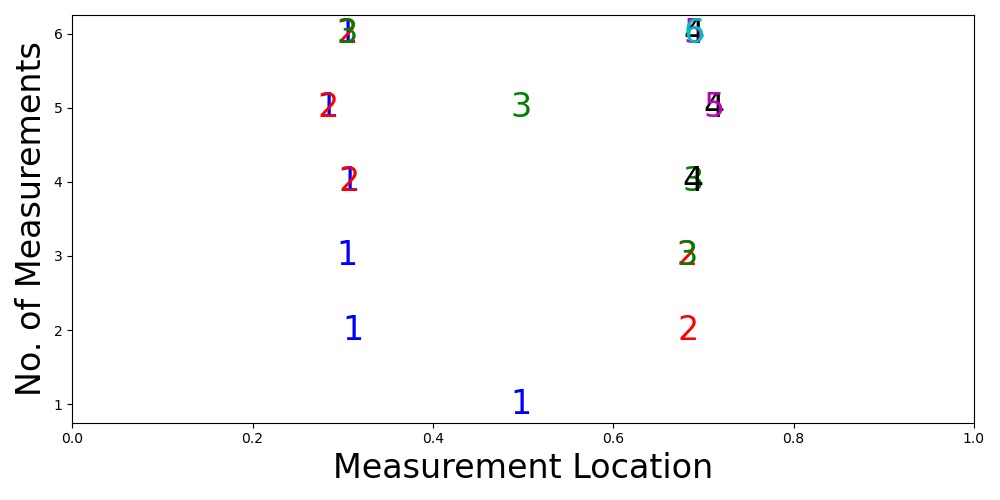
\includegraphics[height=0.5\textwidth]{figs/example.png}
%DIFDELCMD <     %%%
\DIFdelendFL \DIFaddbeginFL 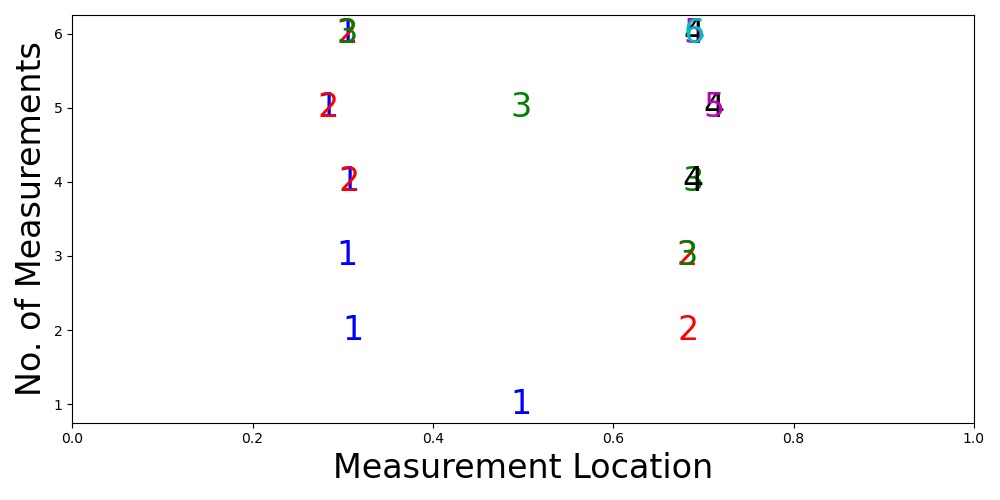
\includegraphics[height=0.5\textwidth]{figs/dst_modelError0.png}
    \DIFaddendFL \caption{Measurement clusterization \DIFdelbeginFL \DIFdelFL{for optimal }\DIFdelendFL \DIFaddbeginFL \DIFaddFL{in D-optimal }\DIFaddendFL designs \DIFdelbeginFL \DIFdelFL{when
      inverting }\DIFdelendFL for the
      \DIFdelbeginFL \DIFdelFL{initial condition }\DIFdelendFL \DIFaddbeginFL \DIFaddFL{inverse problem }\DIFaddendFL of the 1D heat equation\DIFdelbeginFL \DIFdelFL{(see
      supplementary material for details)}\DIFdelendFL . Measurement locations
      were chosen according to the Bayesian D-optimality criterion of
      Theorem \ref{thm:d_optimality}. Measurement locations are
      plotted over the computational domain \(\Omega = [0, 1]\)
      (x-axis), for varying numbers of measurements (y-axis). The
      colored numbers are measurement indices, plotted for visual
      clarity. Measurement clusterization already occurs for three
      measurements: the second measurement (red) is overlaid \DIFdelbeginFL \DIFdelFL{with }\DIFdelendFL \DIFaddbeginFL \DIFaddFL{on }\DIFaddendFL the
      third (green). For five measurements, first (blue) and second
      (red) measurements are clustered, as well as the fourth (black)
      and the fifth (magenta).}
  \label{fig:clusterization_illustration}
\end{figure}


\DIFdelbegin \DIFdel{Researchers }\DIFdelend \DIFaddbegin \DIFadd{Clusterization should not be confused with either repetition nor with
replication, which are commonly viewed as beneficial and even
necessary aspects of an optimal design \mbox{%DIFAUXCMD
\cite{fisher1949design,
  morris2011, schafer2001replication}}\hskip0pt%DIFAUXCMD
. For example,
\mbox{%DIFAUXCMD
\cite{fisher1949design} }\hskip0pt%DIFAUXCMD
in his famous milk and tea experiment,
suggested that repetition is a "way of enlarging the experiment and,
thereby, increasing its sensitiveness". In another example,
\mbox{%DIFAUXCMD
\cite{fay2000rainfall} }\hskip0pt%DIFAUXCMD
measured the effect of rainfall on grass growth
in plots of land. The experiment involved fifteen "rainfall
manipulation shelters", where "Four rainfall manipulation treatments
(three replicates) then were assigned to 12 of the plots". While it
seems reasonable for the researchers to replicate the phenomenon they
are trying to study, clusterization is different: a clustered design
in the rainfall experiment would imply the researchers should take a
repeated measurement }\emph{\DIFadd{on the same plot}}\DIFadd{, at the expense of
measuring grass growth in other plots. In sharp contrast to repetition
and replication, clusterization is highly nonintuitive and we will see
that its origins run considerably deeper.
}


\DIFadd{Researchers of inverse problems }\DIFaddend widely agree that measurement
clusterization is undesirable
\DIFdelbegin \DIFdel{\mbox{%DIFAUXCMD
\cite{fedorov1996, nyberg2012, fedorov1997, Ucinski05,
  neitzel2019sparse}}\hskip0pt%DIFAUXCMD
}\DIFdelend \DIFaddbegin \DIFadd{\mbox{%DIFAUXCMD
\cite{fedorovDesignSpatialExperiments1996, nyberg2012, fedorov1997,
  Ucinski05, neitzel2019sparse}}\hskip0pt%DIFAUXCMD
}\DIFaddend , prompting the exploration of various
remedies to address this issue. One approach involves merging close
measurements \cite{fedorov1997}; however, this strategy merely
overlooks the phenomenon of measurement clusterization. An alternative
solution lies in \emph{clusterization-free design}s, where measurement
locations are deliberately chosen to be distant from one another. This
can be achieved by imposing distance constraints between measurements
or by introducing correlated errors that account for both observation
error and model misspecification \cite{Ucinski05}. For instance, in
the context of time-series analysis for pharmacokinetic experiments,
measurement clusterization can be mitigated by incorporating the
modeling of auto-correlation time within the noise terms
\cite{nyberg2012}.


In spatial problems involving choice of measurements within a domain
\(\Omega \subseteq \mathbb{R}^d, d=1,2,3\), many researchers
circumvent the problem of measurement clusterization by \DIFdelbegin \DIFdel{choosing
measurements from }\DIFdelend \DIFaddbegin \DIFadd{restricting
measurements to }\DIFaddend a coarse grid in \(\Omega\) \cite{koval2020,
  alexanderian2021, attia2022, alexanderian2014, alexanderian2016,
  alexanderian2018efficient, brunton2016}. This approach incurs a
significant computational cost as it requires solving a difficult
combinatorial optimization problem for measurement locations over a
\DIFdelbegin \DIFdel{finite }\DIFdelend \DIFaddbegin \DIFadd{discrete }\DIFaddend set. The combinatorial optimization problem is usually
relaxed by first assigning optimal measurement weights in
\(\mathbb{R}_+\) to the potential measurement locations. Some
researchers incorporate a sparsifying \(\ell_1\) penalty term into the
design criterion, which is subsequently thresholded to achieve the
desired binary design over the coarse grid
\cite{horesh2008borehole}. Others progressively relax the \(\ell_1\)
penalty to an \(\ell_0\) penalty via a continuation method
\cite{alexanderian2016, alexanderian2014}. Others cast the problem of
finding optimal measurement weights as a stochastic optimization
problem \cite{attia2022stochastic}. All of the aforementioned methods
may indeed find a binary optimal design restricted to a given coarse
grid. However, none addresses one fundamental issue: the restriction
of measurement locations to a coarse grid in \(\Omega\) fundamentally
changes the optimal design problem and thus results in a sub-optimal
design.

Avoiding measurement clusterization is a pragmatic approach:
intuitively, researchers recognize that measurement clusterization is
undesirable, even though the underlying reasons may not be fully
clear. Consequently, they strive to prevent it and devise various
methodologies to avoid \DIFdelbegin \DIFdel{measurement clusterization}\DIFdelend \DIFaddbegin \DIFadd{it}\DIFaddend . Yet each and every one of these
methodologies achieves its objective by imposing restrictions on
measurement locations, thereby fundamentally altering the optimal
design problem. To the best of my knowledge, no previous study has
tried to address some seemingly simple yet fundamental questions:
%DIF < 
Why does imposing correlations between observations alleviate
measurement clusterization?
%DIF < 
Is measurement clusterization a generic phenomenon? 
%DIF < 
And, most importantly: Why does measurement clusterization occur?
%DIF < 
%DIF < Should we aim to avoid measurement clusterization?
%DIF < 
%DIF < Is it possible to substitute an optimal clustered design with an
%DIF < equally optimal non-clustered design?
%DIF < Can an optimal clustered design be relpaced with an equally optimal
%DIF < non-clustered design?



\subsection{Contribution}
The primary objective of this study is to provide a \DIFdelbegin \DIFdel{comprehensive
}\DIFdelend \DIFaddbegin \DIFadd{deep }\DIFaddend understanding
of measurement clusterization by addressing the aforementioned
questions. Our focus centers around investigating the Bayesian
D-optimality criterion\DIFdelbegin \DIFdel{, which involves maximizing the
expected Kullback-Leibler divergence between the posterior and prior
measures \mbox{%DIFAUXCMD
\cite{CoverThomas91, Chaloner1995}}\hskip0pt%DIFAUXCMD
}\DIFdelend . We conduct an analysis of Bayesian D-optimal
designs within the context of linear inverse problems over Hilbert
spaces \DIFdelbegin \DIFdel{. We }\DIFdelend \DIFaddbegin \DIFadd{and study two inverse problems: (a) In Sections
\ref{section:prelim} and \ref{section:D_and_grad} we }\DIFaddend propose a novel
\DIFdelbegin \DIFdel{relaxed model for }\DIFdelend \DIFaddbegin \DIFadd{generic model for an inverse problem where }\DIFaddend D-optimality \DIFdelbegin \DIFdel{that }\DIFdelend maintains
analytical tractability and \DIFdelbegin \DIFdel{enables the
identification of }\DIFdelend D-optimal designs \DIFdelbegin \DIFdel{using }\DIFdelend \DIFaddbegin \DIFadd{are identified via
}\DIFaddend Lagrange multipliers. This analytical framework facilitates the
exploration of the questions posed at the end of the previous
paragraph\DIFaddbegin \DIFadd{. We also study (b) the inverse problem of the 1D heat
equation from Section \ref{subsec:toy} above. Investigating both
inverse problems allows us to answer the questions posed in the
previous section}\DIFaddend :

\DIFdelbegin %DIFDELCMD < \begin{figure}
%DIFDELCMD <     \centering
%DIFDELCMD <     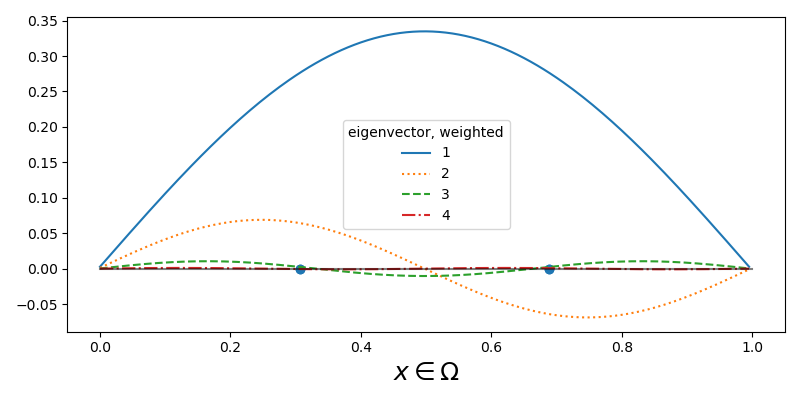
\includegraphics[width=\textwidth]{figs/eigenvectors.png}
%DIFDELCMD <     %%%
%DIFDELCMD < \caption{%
{%DIFAUXCMD
\DIFdelFL{D-optimal measurement locations ($m=4$ measurements) and
      weighted eigenvectors for finding the initial condition of
      the 1D heat equation. Measurement locations and weighted
      eigenvectors are plotted over the computational domain $\Omega =
      [0, 1]$ (x-axis). Measurement clusterization occurs
      approximately at $0.31$ and $0.69$. These two locations are a
      compromise between zeros of eigenvectors a D-optimal design aims
      to ignore (third and up) and staying far from zeros of the
      eigenvectors a D-optimal design aims to measure (first and
      second). Allocating $m=4$ measurements into two locations
      results in clusterization, according to the pigeonhole
      principle.}}
  %DIFAUXCMD
%DIFDELCMD < \label{fig:why}
%DIFDELCMD < \end{figure}
%DIFDELCMD < 

%DIFDELCMD < %%%
\DIFdelend \begin{enumerate}
\DIFdelbegin %DIFDELCMD < 

%DIFDELCMD < %%%
\DIFdelend \item \label{q:generic} \textbf{Is measurement clusterization a
  generic phenomenon?}
%DIF < \subsection{An answer for Question \ref{q:generic}: Genericity of measurement clusterization}
  %DIF < % Computer implementation of Lemma \ref{thm:char} for the inverse
  %DIF < % problem outlined in Section \ref{section:how} also generates \(\obs\)
  %DIF < % as a solution to the D-optimal design problem.  Furthermore,
  \DIFdelbegin \DIFdel{Randomized numerical }\DIFdelend \DIFaddbegin \DIFadd{We give two complementing answers to this question. First, from a
  theoretical perspective, we show that clusterization mainly depends
  on how quickly the eigenvalues of the prior covariance in
  observation space decay. This decay depends mostly on how ill-posed
  the problem at hand is and does not depend much on the prior. See
  Section \ref{section:vanishing} --- particularly, Theorem
  \ref{thm:char} and the discussion following it. We also show results
  of numerical experiments, where }\DIFaddend simulations of our model give rise
  to D-optimal designs that exhibit clusterization \DIFdelbegin \DIFdel{more than 95\% of the time (see
  code in supplementary material). Given our model's genericity}\DIFdelend \DIFaddbegin \DIFadd{with high
  probability in Section \ref{subsec:lemma_sims}. Thus, given the
  genericity of our model}\DIFaddend , we expect measurement clusterization to be
  a generic \DIFaddbegin \DIFadd{and ubiquitous }\DIFaddend phenomenon.

\item \label{q:mitigate} \textbf{Why does imposing correlations
  between observations alleviate measurement clusterization?} In
  Section \ref{section:non_vanishing}, we rigorously demonstrate the
  role of model error in mitigating clusterization, thereby
  corroborating earlier observations made by various
  researchers. \DIFaddbegin \DIFadd{Specifically, our proof shows that identical
  measurements result in no gain in design criterion when observation
  error amplitude tends to zero. Moreover, in Section
  \ref{subsec:corr_errors_sims}, we show that an error term
  corresponding to correlations between measurements mitigates
  clusterization in the inverse problem of the 1D heat equation.
}\DIFaddend 

\item \label{q:why} \textbf{Why does measurement clusterization
  occur?} In \DIFdelbegin \DIFdel{Section \ref{section:why}, we present a compelling explanation for the optimality of clustered designs in the absence
  of model error.
Our analysis reveals that, in our
  model, }\DIFdelend \DIFaddbegin \DIFadd{Sections \ref{subsec:why} we give two compelling answers
  to this question by (i) transporting insights we gain from our
  generic model to the inverse problem of the 1D heat equation, and
  (ii) connecting measurement clusterization to Carath\'eodory's
  Theorem.
}

  \DIFadd{Our analysis for the heat equation relies on conclusions from our
  generic model. In particular, Theorem \ref{thm:char} reveals that }\DIFaddend a
  D-optimal design focuses on a select set of prior eigenvectors,
  \DIFdelbegin \DIFdel{specifically
  }\DIFdelend \DIFaddbegin \DIFadd{i.e.~}\DIFaddend those with the largest eigenvalues in the prior covariance
  spectrum. In practical scenarios, the number of locations where (a)
  \DIFdelbegin \DIFdel{the }\DIFdelend \DIFaddbegin \DIFadd{all }\DIFaddend relevant prior eigenvectors are significantly large, and (b)
  other eigenvectors are close to zero, is limited. Consequently, the
  clusterization of measurements arises as a natural consequence of
  the pigeonhole principle, as there are more measurements available
  than there are locations satisfying conditions (a) and (b).
\DIFdelbegin \DIFdel{See
  Fig~\ref{fig:why}.
}\DIFdelend 

  %DIF < % In Section \ref{section:vanishing}, we provide an insightful
  %DIF < % explanation for the optimality of clustered designs when no model
  %DIF < % error is present. We demonstrate that for our model, a D-optimal
  %DIF < % design measures only a small subset of prior eigenvectors, which are
  %DIF < % the prior eigenvectors with largest power spectrum. In real-life
  %DIF < % problems there are limited number of locations where: (a) the
  %DIF < % relevant prior eigenvectors are large, and other prior eigenvectors
  %DIF < % with large power in the prior spectrum are zero. Then measurement
  %DIF < % clusterization is a result of the pigeonhole principle, where there
  %DIF < % are more measurements than measurement locations satisfying (a) and
  %DIF < % (b).
\DIFaddbegin \DIFadd{The connection to Carath\'eodory's Theorem also utilizes the
  concentration of measurement effort on the abovementioned select set
  of prior eigenvectors. This concentration allows us to move from an
  infinite-dimensional setting to finite dimensions, where the
  conditions of Carath\'eodory's Theorem hold. We conclude that a
  D-optimal design arises by weighting a small number of
  measurements. If the number of allowed measurements is larger than
  the small number dictated by Carath\'eodory's Theorem, we have
  excessive weight on some measurements, which can be interpreted as
  clusterization.
  }\DIFaddend 

%DIF < % We conjecture that the prevalence of measurement clusterization
  %DIF < % arises due to the ease of discovering clustered designs.
\DIFdelbegin %DIFDELCMD < 

%DIFDELCMD < %%%
%DIF < % \item \label{q:avoid} \textbf{Should we aim to avoid measurement
%DIF < %   clusterization?} Based on the analysis conducted in this study, we
%DIF < %   did not find any compelling reason to explicitly avoid optimal
%DIF < %   clustered designs.
%DIFDELCMD < 

%DIFDELCMD < %%%
%DIF < % \item \label{q:replace} \textbf{Is it possible to substitute an
%DIF < %   optimal clustered design with an equally optimal non-clustered
%DIF < %   design?} In Section \ref{section:vanishing}, we answer this question
%DIF < %   in the affirmative, although we show that numerical experiments
%DIF < %   conducted using our model indicate a strong preference for clustered
%DIF < %   designs.
%DIFDELCMD < 

%DIFDELCMD < %%%
\DIFdelend \end{enumerate}
\DIFdelbegin %DIFDELCMD < 

%DIFDELCMD < %%%
\DIFdel{The cornerstone of our investigation into measurement clusterization
is Theorem \ref{thm:char} proven in Section
\ref{section:vanishing}. The key insight of
  Theorem \ref{thm:char}
lies in its fifth component, which highlights that }\DIFdelend \DIFaddbegin 

\subsubsection{\DIFadd{Implications}}
\DIFadd{Our answer to Question \ref{q:generic} implies that encountering
clusterization should be expected in many different problems across
many different scientific fields. Researchers that encounter
clusterization should not be surprised or wary. In Our answer to
Question \ref{q:why}, we explain what our view of the cause of
clusterization is. It appears, the cause is generic: }\DIFaddend a D-optimal
design \DIFdelbegin \DIFdel{aims to uniformly reduce posterior uncertainties for posterior
covariance
eigenvectors in observation space. A similar conclusion was
reached by Koval et al.~\mbox{%DIFAUXCMD
\cite{koval2020}}\hskip0pt%DIFAUXCMD
,
who showed that
A-optimal
designs are best constructed in the space of observations}\DIFdelend \DIFaddbegin \DIFadd{reduces uncertainty for a select set of prior covariance
eigenvectors --- those with the most prior uncertainty, i.e.~those the
practitioner cares about the most! We believe practitioners should not
try to avoid measurement clusterization. Rather, practitioners should
take repeated measurements (e.g.~in MRI and borehole tomography),
increase apparatus sensitivity (e.g.~in EIT), or take consecutive
measurements (e.g.~in the 1D heat equation). Overall, we show that
measurement clusterization is a natural and (almost) inevitable part
of Bayesian D-optimal designs (but see disclaimer below).
}

\DIFadd{One interesting implication of the analysis presented here is that
clusterization can serve as an evidence to the number of relevant
eigenvectors. Since leading eigenvectors typically correspond to slow
variations in space and/or time, clusterization could be used to
estimate the number of relevant degrees of freedom, and even to reduce
the complexity of a computational model, e.g.~by dropping
discretization points}\DIFaddend .

\DIFdelbegin \DIFdel{Before we state Theorem \ref{thm:char} we give some definitions: Let
\(\hilp, \hilo\) Hilbert spaces,
\(\fwd:\hilp \to \hilo\) a linear
compact operator. Let \(\obs: \hilo \to \mathbb{R}^m\) a linear
measurement operator, where \(m \in \mathbb{N}\) is the number of measurements taken. Let \(\sigma^2 \in \mathbb{R}_{+}\) observation
noise variance, \(\data = \obs \fwd \param + \eps\), where \(\eps \in
\mathbb{R}^m\) is iid \(\mathcal{N}(0, \sigma^2)\) noise. Let \(\pr
\sim \mathcal{N}(\prmean, \prcov)\) prior Gaussian measure on
\(\hilp\), where \(\prcov\) is the prior covariance operator and let
\(\post\) the posterior (Gaussian)
measure. }%DIFDELCMD < 

%DIFDELCMD < \begin{theorem}\label{thm:char}
%DIFDELCMD <   %%%
\DIFdel{Let: }%DIFDELCMD < \begin{itemize}
%DIFDELCMD <     \item %%%
\DIFdel{The }\DIFdelend \DIFaddbegin \DIFadd{It is important to note that we do not view clustered designs as
undesirable, nor do we believe it should be avoided at
all. Clusterization is a peculiar phenomenon and it is perfectly
reasonable for someone to argue against the }\DIFaddend D-optimality \DIFdelbegin \DIFdel{design criterion
    \mbox{%DIFAUXCMD
\cite{AlexanderianGloorGhattas14}}\hskip0pt%DIFAUXCMD
:
    }%DIFDELCMD < \begin{align*}
%DIFDELCMD <       \begin{split}
%DIFDELCMD <         \tar(\obs) %:&= \mathbb{E}_{\data}\left [ D_{\text{KL}} (\post || \pr ) \right ] \\
%DIFDELCMD <         % 
%DIFDELCMD <         % 
%DIFDELCMD <         % 
%DIFDELCMD <         &= \frac{1}{2} \log \det ( I + \sigma^{-2} \prcov^{1/2} \fwd ^*
%DIFDELCMD <         \obs^* \obs \fwd \prcov^{1/2}), 
%DIFDELCMD <       \end{split}
%DIFDELCMD <     \end{align*}
%DIFDELCMD <   \item %%%
\DIFdel{\(\obs\) a D-optimal design operator
    }%DIFDELCMD < \begin{equation*}
%DIFDELCMD <       \obs = \argmax_{\|\meas_j\| = 1, j=1,\dots,m}\tar(\obs),
%DIFDELCMD <     \end{equation*}
%DIFDELCMD <   \item %%%
\DIFdel{\(\{\lambda_i\}_{i=1}^\infty\) eigenvalues of \(\fwd\prcov\fwd^*\) in decreasing order of magnitude. %DIF < % \item \(\{\ev_i\}_{i=1}^\infty\) their corresponding eigenvectors.
  }%DIFDELCMD < \item %%%
\DIFdel{\(\{\eta_i\}_{i=1}^\infty\) eigenvalues of \(\obs^*\obs\). }\DIFdelend \DIFaddbegin \DIFadd{criterion
based on the fact that it results in clustered designs. We have seen,
however that there is a perfectly reasonable explanation for
clusterization. We have shown that clusterization is an inevitable
consequence of having a problem with some modes where uncertainty
decays faster than others.
}\DIFaddend 

\DIFdelbegin %DIFDELCMD < \end{itemize}
%DIFDELCMD < %%%
\DIFdelend \DIFaddbegin \DIFadd{Lastly, we believe that when clusterization arises, it should serve as
a warning sign to practitioners. In the inverse problem of the 1D heat
equation, clusterization occurs primarily because Laplacian
eigenvectors }\emph{\DIFadd{do not}} \DIFadd{decay in $\Omega$. Consequently, measuring
$u(x_1, T)$ at some point $x_1 \in \Omega$ provides information about
$u(x_2,T)$ for distant points $x_2 \in \Omega$. Intuitively, this
should not occur: for small $T$, the heat distribution at $x_1$ should
give very little knowledge on the heat distribution at $x_2$. This
behavior stems from a well-known property of the heat equation: it
allows information to spread }\emph{\DIFadd{instantly}} \DIFadd{across the computational
domain \mbox{%DIFAUXCMD
\cite{renardy2006PDE}}\hskip0pt%DIFAUXCMD
. In reality, heat (and information)
propagate at finite speeds. Of course, the known physical barrier for
information spread is the speed of light, but we expect heat to spread
considerably slower: heating an Olympic pool at one end should have no
immediate effect on the temperature at the other end.
}\DIFaddend 

\DIFdelbegin \DIFdel{Then:
  }%DIFDELCMD < \begin{enumerate}
\begin{enumerate}%DIFAUXCMD
%DIFDELCMD <   \item  %%%
\item%DIFAUXCMD
\DIFdel{\(\tr{\obs^*\obs} = m\).
}%DIFDELCMD < \item %%%
\item%DIFAUXCMD
\DIFdel{\(\obs^*\obs\) and \(\fwd\prcov\fwd^*\) are simultaneously
    diagonalizable. }%DIFDELCMD < \item %%%
\item%DIFAUXCMD
\DIFdel{\(k := \rank \obs^*\obs \leq m\) and
}%DIFDELCMD < \begin{equation*}
%DIFDELCMD <       \tar(\obs) = \frac{1}{2} \sum_{i=1}^{k} \log (1 + \sigma^{-2}\lambda_i\eta_i). %= \frac12 \sum_{i=1}^{m} \log (1 + \sigma^{-2}\lambda_i\eta_i).
%DIFDELCMD <     \end{equation*}
%DIFDELCMD <   %%%
%DIF < % \item 
  %DIF < %   \begin{equation*}
  %DIF < %     k = \argmax \left \{ k:\lambda_k^{-1} < \sigma^{-2}\frac{m}{k} + \frac{1}{k} \sum_{j=1}^{k}
  %DIF < %     \lambda_j^{-1} \right \}.
  %DIF < %   \end{equation*}
  %DIFDELCMD < \item
\item%DIFAUXCMD
%DIFDELCMD <     \begin{equation*}
%DIFDELCMD <         \eta_i = \begin{cases}
%DIFDELCMD <           \frac{m}{k} - \sigma^2 \lambda_i^{-1} + \sigma^2 \frac{1}{k} \sum_{j=1}^k \lambda_j^{-1} & 1 \leq i \leq k \\
%DIFDELCMD <           0 & i > k 
%DIFDELCMD <         \end{cases}.
%DIFDELCMD <     \end{equation*}
%DIFDELCMD <   \item %%%
\item%DIFAUXCMD
\DIFdel{The covariance of the pushforwad \(\fwd_{*} \post\) is \(\left
    ( (\fwd \prcov \fwd^*)^{-1} + \sigma^{-2} \obs^*\obs \right
    )^{-1}\) and its eigenvalues are
}%DIFDELCMD < \begin{equation*}
%DIFDELCMD <       \theta_i =
%DIFDELCMD <       \begin{cases}
%DIFDELCMD <         \left(\frac{\sum_{j=1}^k \lambda_j^{-1} + \sigma^{-2}m}{k} \right )^{-1} & i \leq k \\
%DIFDELCMD <         \lambda_i &  i > k 
%DIFDELCMD <       \end{cases}
%DIFDELCMD <     \end{equation*}

\end{enumerate}%DIFAUXCMD
%DIFDELCMD <   \end{enumerate}
%DIFDELCMD < \end{theorem}
%DIFDELCMD < %%%
\DIFdelend \DIFaddbegin \DIFadd{Our choice of prior is also a potential major contributor to
clusterization. Our choice of Gaussian prior similarly implies
information is shared between distant locations in $\Omega$. Thus, we
suggest refraining from choosing Gaussian priors with inverse
Laplacian covariance operators. Rather, non-Gaussian priors could be
employed instead \mbox{%DIFAUXCMD
\cite{hosseini2017, hosseini2019}}\hskip0pt%DIFAUXCMD
.
}\DIFaddend 

\DIFaddbegin \DIFadd{We believe that the emergence of clusterization in this context is
thus non-physical, arising from the way the inverse problems we
consider are phrased. Clusterization therefore indicates that the
underlying mathematical / Bayesian model is overly permissive and
fails to capture crucial physical constraints of the problem. We
suggest that when clusterization occurs, practitioners should consider
alternative models where information is localized in space and travels
at finite speed in the medium. Such models may not only provide more
physically accurate and meaningful results but may also mitigate the
issue of clusterization.
}



\subsubsection{\DIFadd{Other Contributions}}
\DIFadd{In Theorem \ref{thm:char}, we also show that D-optimal designs are
best understood in the space of }\emph{\DIFadd{observations}}\DIFadd{, see Section
\ref{section:vanishing} for a precise statement. This is in accordance
with previous work by \mbox{%DIFAUXCMD
\cite{koval2020}}\hskip0pt%DIFAUXCMD
, who showed that A-optimal
designs are best constructed in the space of observations.
}

\DIFaddend In the process of proving Theorem \ref{thm:char} we prove and
generalize several lemmas. Among those, is Lemma \ref{lemma:free},
which is (to the the best of my knowledge) \DIFdelbegin \DIFdel{a novellemma in linear
algebra}\DIFdelend \DIFaddbegin \DIFadd{novel}\DIFaddend : We decompose a
symmetric positive definite matrix \(M \in \mathbb{R}^{k \times k}\)
with \(\ttr M = m \in \mathbb{N}\) as \(M = AA^t\), where \DIFdelbegin \DIFdel{\(A\) }\DIFdelend \DIFaddbegin \DIFadd{\(A\in
\mathbb{R}^{k \times m}\) }\DIFaddend has unit norm columns.


%DIF < % Finally, in Lemma \ref{lemma:lax} we generalize a lemma for
%DIF < % calculating \(\frac{\der}{\der t} \log \det (I + X(t))\), where
%DIF < % \(X(t)\)is an operator valued function \cite{Lax07}.
\DIFdelbegin %DIFDELCMD < 

%DIFDELCMD < %%%
\DIFdelend \subsection{Limitations}\label{subsec:limitations}
The main limitation of this study is that our generic model does not
correspond to any specific real-life problem. \DIFdelbegin \DIFdel{It }\DIFdelend \DIFaddbegin \DIFadd{Specifically, in its
current form, our model does not allow point evaluations. Thus, while
our model }\DIFaddend is generic enough to be analytically tractable, \DIFdelbegin \DIFdel{but one may
argue }\DIFdelend \DIFaddbegin \DIFadd{some may
argue that }\DIFaddend our model is too far removed from any real application. To
these claims I would answer that scientists have a long history of
studying models that are bare-bones simplifications of real systems,
e.g.\DIFaddbegin \DIFadd{~}\DIFaddend the Ising model \cite{cipra1987}, the Lorenz system \cite{brin},
the Lotka-Volterra equations \cite{logan2006}, the Carnot engine
\cite{kardar2007} \DIFdelbegin \DIFdel{, }\DIFdelend and many others.
 \section{Preliminaries and Notation}\label{section:prelim}
\DIFdelbegin %DIFDELCMD < 

%DIFDELCMD < %%%
\DIFdel{In this section }\DIFdelend \DIFaddbegin \DIFadd{Here }\DIFaddend we present the \DIFdelbegin \DIFdel{setup that will be used throughout this
article. The theoretical }\DIFdelend \DIFaddbegin \DIFadd{basics of Bayesian inverse problems over Hilbert
spaces. Since we are ultimately interested in inferring a function
over some domain, we will keep in mind that these Hilbert spaces
should really be thought of as function spaces. A deeper treatment of
the }\DIFaddend foundations for inverse problems over function spaces can be found
\DIFdelbegin \DIFdel{elsewhere \mbox{%DIFAUXCMD
\cite{Stuart10}}\hskip0pt%DIFAUXCMD
and will not be
reviewed here}\DIFdelend \DIFaddbegin \DIFadd{in \mbox{%DIFAUXCMD
\cite{Stuart10}}\hskip0pt%DIFAUXCMD
}\DIFaddend .


\subsection{\DIFdelbegin \DIFdel{Bayesian Linear Inverse }\DIFdelend \DIFaddbegin \DIFadd{Forward }\DIFaddend Problems}\label{subsec:abstract_OED}
\DIFdelbegin \DIFdel{Let }\DIFdelend \DIFaddbegin \DIFadd{In this section we give definitions and notations for forward problems,
which are an essential part of the inverse problems we discuss
later. Consider a "parameter space" }\DIFaddend \(\hilp\) and \DIFaddbegin \DIFadd{an "observation
space" }\DIFaddend \(\hilo\) \DIFaddbegin \DIFadd{--- both }\DIFaddend separable Hilbert spaces (the subscripts p
and o are for "parameter" and "observation", respectively)\DIFdelbegin \DIFdel{, and let
\(\fwd: \hilp \to \hilo\) }\DIFdelend \DIFaddbegin \DIFadd{. The
parameter space includes the quantity we seek to infer; in the inverse
problem of the heat equation, the parameter space $\hilp$ is where the
initial condition lives. The observation space $\hilo$, on the other
hand, is the space from which we take measurements; in the example of
the 1D heat equation, $u(\cdot, T) \in \hilo$.
}

\DIFadd{The connection between parameter and observation spaces is made by }\DIFaddend the
\emph{forward operator} \DIFdelbegin \DIFdel{. The }\DIFdelend \DIFaddbegin \DIFadd{\(\fwd: \hilp \to \hilo\). We assume the
}\DIFaddend forward operator \(\fwd\) is \DIFdelbegin \DIFdel{assumed linearand strongly smoothing (the heat
operator }\DIFdelend \DIFaddbegin \DIFadd{linear. In the inverse problem }\DIFaddend of the 1D
heat equation\DIFdelbegin \DIFdel{introduced in Section
\ref{section:intro} is a prime example). Take a Gaussian prior
\(\param \sim \pr = \normal(\prmean ,\prcov)\) with some appropriate
covariance operator \(\prcov\) on \(\hilp\) \mbox{%DIFAUXCMD
\cite{Stuart10}}\hskip0pt%DIFAUXCMD
. Note that
\(\fwd \prcov \fwd^*\) is the prior covariance in \(\hilo\)
\mbox{%DIFAUXCMD
\cite{Stuart10}}\hskip0pt%DIFAUXCMD
, and
as such, \(\fwd \prcov \fwd^*\) is assumed
invertible --- an assumption which will be used below (if \(\fwd\) has
a nontrivial kernel we utilize Occam's Razor and ignore said kernel
altogether).
}\DIFdelend \DIFaddbegin \DIFadd{, the forward operator is determined by the time
evolution of the 1D heat equation \eqref{eq:heat1} and
\eqref{eq:heat2}, so $u(\cdot, T) = \fwd u_0$.
}

\DIFaddend Measurements are taken via a \DIFaddbegin \DIFadd{linear }\DIFaddend \emph{measurement operator}
\(\obs\)\DIFdelbegin \DIFdel{. It is common for the measurement and forward operators to be
merged \(\tmp := \obs \fwd\) \mbox{%DIFAUXCMD
\cite{AlexanderianGloorGhattas14}}\hskip0pt%DIFAUXCMD
, but
the analysis carried out in the following sections requires that
\(\fwd\) and \(\obs\) are explicitly separated as in
\mbox{%DIFAUXCMD
\cite{attia2022stochastic, cvetkovic2023choosing}}\hskip0pt%DIFAUXCMD
.  }\DIFdelend \DIFaddbegin \DIFadd{, which is the concatenation of linear functionals
$\meas_1,\dots,\meas_m$ we call }\emph{\DIFadd{measurements}}\DIFadd{:
}\begin{equation*}\obs u = (\meas_1(u), \dots, \meas_m(u) )^t \in \R^m,\ u \in \hilo.
\end{equation*}
\DIFadd{Thus, }\DIFaddend \(\obs \in ( \hilo^* )^m\), where \(m\) is the number of
measurements taken\DIFdelbegin \DIFdel{. Entries \(\meas_j, j=1,\dots,m\) of the observation operator
\(\obs\) are called }\emph{\DIFdel{measurements}}%DIFAUXCMD
\DIFdel{:
}\DIFdelend \DIFaddbegin \footnote{\DIFadd{The alert reader will likely ask how do we
reconcile point measurements $\delta_x$ as suggested by the
formulation of the 1D heat equation with working in Hilbert spaces. We
don't. We follow standard practice in the literature and restrict our
analysis to Hilbert spaces. We can satisfy ourselves with the fact
that point evaluations could be approximated in a standard Hilbert
space like $L^2(\Omega)$.}}\DIFadd{.
}\DIFaddend 

\DIFdelbegin %DIFDELCMD < \begin{equation*}%\label{eq:O}
%DIFDELCMD <   \obs u = (\meas_1(u), \dots, \meas_m(u) )^t \in \R^m,\ u \in \hilo.
%DIFDELCMD < \end{equation*}
%DIFDELCMD < 

%DIFDELCMD < %%%
\DIFdelend Data is acquired via noisy observations, and we consider two types of
error terms: Spatially correlated model error \(\eps' \sim
\normal(0,\modcov)\) with \(\modcov\) a covariance operator\DIFdelbegin \DIFdel{. Observation
error is }\DIFdelend \DIFaddbegin \DIFadd{; and
observation error }\DIFaddend denoted \(\eps \sim \normal(0, \sigma^2 I_m)\), with
\(I_m \in \mathbb{R}^{m \times m}\) the identity. Both error terms and
the prior \DIFaddbegin \DIFadd{(see Section \ref{subsec:bayesian_inverse_problems} below)
}\DIFaddend are assumed independent of each other. Thus, data is acquired via
\begin{align}\label{eq:inverse_problem}
  \data := \obs (\fwd \param + \eps') + \eps = \obs \fwd \param + \obs \eps' + \eps.
\end{align}

It is easy to verify that \(\obs \eps' + \eps \in \R^m\) is a centered
Gaussian random vector with covariance matrix

\DIFdelbegin %DIFDELCMD < \begin{align}\label{eq:Sigma}
%DIFDELCMD <   \begin{split}
%DIFDELCMD <     \Sigma(\obs) :&= \mathbb{E}[ (\obs \eps' + \eps) (\obs \eps' +
%DIFDELCMD <       \eps)^t ]
%DIFDELCMD <     % 
%DIFDELCMD <     % 
%DIFDELCMD <     = \obs \modcov \obs^* + \sigma^2I_m , 
%DIFDELCMD <   \end{split}
%DIFDELCMD < \end{align}%%%
\DIFdelend \DIFaddbegin \begin{align}\label{eq:Sigma}
  \begin{split}
    \Sigma(\obs) :&= \mathbb{E}[ (\obs \eps' + \eps) (\obs \eps' +
      \eps)^t ]
= \obs \modcov \obs^* + \sigma^2I_m , 
  \end{split}
\end{align}\DIFaddend 
where
\DIFdelbegin %DIFDELCMD < \begin{align}\label{eq:modcov_explained}
%DIFDELCMD <   \begin{split}
%DIFDELCMD <     [\obs \modcov \obs^*]_{ij} & = e_i^t \obs \modcov \obs^* e_j 
%DIFDELCMD <     %
%DIFDELCMD <     %
%DIFDELCMD <     %
%DIFDELCMD <     = \meas_i (\modcov \meas_j).% \text{ (by \eqref{eq:obs*})}.
%DIFDELCMD <   \end{split}
%DIFDELCMD < \end{align}%%%
\DIFdelend \DIFaddbegin \begin{align}\label{eq:modcov_explained}
  \begin{split}
    [\obs \modcov \obs^*]_{ij} & = e_i^t \obs \modcov \obs^* e_j 
= \meas_i (\modcov \meas_j).\end{split}
\end{align}\DIFaddend 
Taking \(\modcov = 0\) is a common practice
\DIFdelbegin \DIFdel{\mbox{%DIFAUXCMD
\cite{tarantola2005,Kaipio2005,Vogel02} }\hskip0pt%DIFAUXCMD
}\DIFdelend \DIFaddbegin \DIFadd{\mbox{%DIFAUXCMD
\cite{tarantola2005,kaipio2005,Vogel02} }\hskip0pt%DIFAUXCMD
}\DIFaddend and then \(\Sigma =
\sigma^2I_m\) is a scalar matrix which does not depend on \(\obs\).

\DIFdelbegin \DIFdel{Finally, it is
useful to record that the posterior measure }\DIFdelend \DIFaddbegin \subsection{\DIFadd{Bayesian Linear Inverse Problems}}\label{subsec:bayesian_inverse_problems}
\DIFadd{In the previous section, we saw how a parameter $u\in \hilp$ is
transported to the observation space via the forward operator $\fwd u
\in \hilo$, how observations are generated from a parameter via $\obs
\fwd u$ and how observations and noise give rise to data $\data$. It
is time to formulate the process of inferring the parameter as a
Bayesian inverse problem. We have already defined the likelihood in
the previous section, and now we will define the prior.
}

\DIFadd{We take a Gaussian prior \(\param \sim \pr = \normal(\prmean
,\prcov)\) with some appropriate covariance operator \(\prcov\) on
\(\hilp\) \mbox{%DIFAUXCMD
\cite{Stuart10}}\hskip0pt%DIFAUXCMD
. For example, for the inverse problem of the
1D heat equation we chose $\prcov = (-\Delta)^{-1}$, as described in
Section \ref{subsec:toy}. Note that \(\fwd \prcov \fwd^*\) is the
prior covariance in \(\hilo\) \mbox{%DIFAUXCMD
\cite{Stuart10}}\hskip0pt%DIFAUXCMD
, and as such is assumed
invertible --- an assumption which we will use later (if \(\fwd\) has
a nontrivial kernel we utilize Occam's Razor and ignore said kernel
altogether).
}

\DIFadd{Since $\fwd$ is linear and $\pr$ is Gaussian --- the posterior
}\DIFaddend \(\post\) is Gaussian \DIFdelbegin \DIFdel{in this setting and its covariance operator does not
depend on data \(\data\) }\DIFdelend \DIFaddbegin \DIFadd{as well. We do not utilize the posterior mean in
this study, but the posterior covariance operator $\postcov$ is given
by the known formula }\DIFaddend \cite{Stuart10}:
\begin{align}\label{eq:postcov}
  \postcov = (\prcov^{-1} + \fwd^* \obs^* \Sigma^{-1} \obs \fwd
  )^{-1}.
\end{align}

\subsection{Bayesian D-Optimal Designs\DIFdelbegin \DIFdel{in Infinite Dimensions}\DIFdelend }\label{subsec:D_optimal_design} 
A Bayesian D-optimal design maximizes \DIFdelbegin \DIFdel{expected Kullback-Leibler (KL )
}\DIFdelend \DIFaddbegin \DIFadd{the expected KL }\DIFaddend divergence
between posterior \(\post\) and prior measures \(\pr\). \DIFdelbegin \DIFdel{It is
useful to first recall the definition of KL divergence \mbox{%DIFAUXCMD
\cite{CoverThomas91}}\hskip0pt%DIFAUXCMD
}\DIFdelend \DIFaddbegin \DIFadd{For arbitrary
posterior and prior measures, the KL divergence is defined,
analogously to eq.~\eqref{eq:basic_KL}, via the Radon-Nikodym
derivative}\DIFaddend :
\begin{equation*}
  D_{KL}(\post||\pr) = \int \log \frac{\der \post}{\der \pr}(\param) \der \post(\param).
\end{equation*}

The study of D-optimal designs for Bayesian linear inverse problems in
infinite dimensions was pioneered by \cite{AlexanderianGloorGhattas14,
  alexanderian2018efficient}. The main result we will make use of is
summarized (in our notation) below:

\begin{theorem}[Alexanderian, Gloor, Ghattas \cite{AlexanderianGloorGhattas14}]\label{thm:d_optimality}
  Let \(\pr = \normal(\prmean,\prcov)\) be a Gaussian prior on \(\hilp\)
  and let \(\post = \normal(\postmean,\postcov)\) the posterior measure
  on \(\hilp\) for the Bayesian linear inverse problem \(\data = \obs
  \fwd\param + \obs \eps' + \eps\) discussed above. Then
  \DIFdelbegin %DIFDELCMD < \begin{align}\label{eq:objective}
%DIFDELCMD <     \begin{split}
%DIFDELCMD <       \tar( \obs) :&= \mathbb{E}_{\data}\left [ D_{\text{KL}} (\post || \pr ) \right ] \\
%DIFDELCMD <       % 
%DIFDELCMD <       % 
%DIFDELCMD <       % 
%DIFDELCMD <       &= \frac{1}{2} \log \det 
%DIFDELCMD <       ( I + \prcov^{1/2}  \fwd ^* \obs^* \Sigma^{-1} \obs \fwd \prcov^{1/2}).
%DIFDELCMD <     \end{split}
%DIFDELCMD <   \end{align}%%%
\DIFdelend \DIFaddbegin \begin{align}\label{eq:objective}
    \begin{split}
      \tar( \obs) :&= \mathbb{E}_{\data}\left [ D_{\text{KL}} (\post || \pr ) \right ] \\
&= \frac{1}{2} \log \det 
      ( I + \prcov^{1/2}  \fwd ^* \obs^* \Sigma^{-1} \obs \fwd \prcov^{1/2}).
    \end{split}
  \end{align}\DIFaddend 
\end{theorem}

\DIFdelbegin \DIFdel{Note that in }\DIFdelend \DIFaddbegin \DIFadd{In }\DIFaddend \cite{AlexanderianGloorGhattas14, alexanderian2018efficient},
results are stated for \(\Sigma=I\) (implied by \(\modcov =
0,\sigma^2=1\)), but these results also hold for more general
covariance matrices \cite[p. 681]{AlexanderianGloorGhattas14}.

%DIF < % It is important to note that since \(\obs\) is finite-rank,
%DIF < % \(\prcov^{1/2} \fwd ^* \obs^* \Sigma^{-1} \obs \fwd \prcov^{1/2}\) is
%DIF < % trace-class.
\begin{definition}\label{def:d_optimality}
  We say \DIFdelbegin \DIFdel{\(\obs^{\star}\) }\DIFdelend \DIFaddbegin \DIFadd{\(\opt\) }\DIFaddend is \emph{D-optimal} if \DIFdelbegin \DIFdel{\(\obs^{\star} =
  \argmax_{\obs} \tar(\obs)\)}\DIFdelend \DIFaddbegin \DIFadd{\(\opt =
  \argmax_{\obs} \tar(\obs)\)}\DIFaddend , where entries of \(\obs \in (\hilo^*)^m\)
  are constrained to some allowed set of measurements in \(\hilo^*\).
\end{definition}

Intuition for Theorem \ref{thm:d_optimality} can be gained by
\DIFdelbegin \DIFdel{considering }\DIFdelend \DIFaddbegin \DIFadd{recalling from Section \ref{subsec:D} that for }\DIFaddend a Bayesian linear model
in finite dimensions, with Gaussian prior and Gaussian noise\DIFdelbegin \DIFdel{. Then}\DIFdelend , a
D-optimal design minimizes the determinant of the posterior covariance
matrix\DIFdelbegin \DIFdel{, and this turns out
to be a regularized version of the frequentist D-optimality criterion
\mbox{%DIFAUXCMD
\cite{Chaloner1995}}\hskip0pt%DIFAUXCMD
}\DIFdelend . Theorem
\ref{thm:d_optimality} and Definition \ref{def:d_optimality} carry a
similar intuition:
\DIFdelbegin %DIFDELCMD < \begin{align*}
%DIFDELCMD <   \begin{split}
%DIFDELCMD <     \tar(\obs) &= \frac{1}{2} \log \det ( I + \prcov^{1/2}  \fwd ^* \obs^* \Sigma^{-1} \obs \fwd \prcov^{1/2}) \text{ by \eqref{eq:objective}}\\
%DIFDELCMD <     &= \frac{1}{2} \log \det \Big( \prcov ( \prcov^{-1} + \fwd ^* \obs^* \Sigma^{-1} \obs \fwd) \Big )\\
%DIFDELCMD <     &= \frac{1}{2} \log \det \prcov \postcov^{-1} \text{ by \eqref{eq:postcov}}.
%DIFDELCMD <     %%  &= \frac12 \log \det \prcov -\frac12 \log \det \postcov.
%DIFDELCMD <   \end{split}
%DIFDELCMD < \end{align*}%%%
\DIFdelend \DIFaddbegin \begin{align*}
  \begin{split}
    \tar(\obs) &= \frac{1}{2} \log \det ( I + \prcov^{1/2}  \fwd ^* \obs^* \Sigma^{-1} \obs \fwd \prcov^{1/2}) \text{ by \eqref{eq:objective}}\\
    &= \frac{1}{2} \log \det \Big( \prcov ( \prcov^{-1} + \fwd ^* \obs^* \Sigma^{-1} \obs \fwd) \Big )\\
    &= \frac{1}{2} \log \det \prcov \postcov^{-1} \text{ by \eqref{eq:postcov}}.
\end{split}
\end{align*}\DIFaddend 
We think of \(\prcov\) as constant, \DIFdelbegin \DIFdel{so }\DIFdelend \DIFaddbegin \DIFadd{in the sense that $\prcov$ does
not depend on data $\data$. Thus, }\DIFaddend a D-optimal design minimizes a
quantity analogous to the posterior covariance determinant, similarly
to the finite-dimensional case.











 %DIF < % \subsection{Notation Summary}\label{subsec:notation}
%DIF < %   Our notation is summarized below. We let:
%DIF < %   \begin{itemize}
%DIF < %   \item \(\hilp, \hilo\) Hilbert spaces.
%DIF < %   \item \(\fwd:\hilp \to \hilo\) a linear compact operator.
%DIF < %   \item \(\pr \sim \mathcal{N}(0, \prcov)\) prior Gaussian measure on
%DIF < %     \(\hilp$, with prior covariance operator \(\prcov:\hilp \to \hilp$.
%DIF < %   \item \(\obs: \hilo \to \mathbb{R}^m\) measurement operator, where \(m
%DIF < %     \in \mathbb{N}\) is the number of measurements taken.
%DIF < %   \item \(\sigma^2 \in \mathbb{R}_{+}\) observation noise variance.
%DIF < %   \item \(\modcov\) model error covariance operator.
%DIF < %     %% \(\data = \obs \fwd \param + \eps$, where \(\eps \in
%DIF < %     %% \mathbb{R}^m\) isiid \(\mathcal{N}(0, \sigma^2)\) noise.
%DIF < %   \item \(\Sigma(\obs) = \obs \modcov \obs^* + \sigma^2I$. 
%DIF < %   \item \(\post\) the posterior measure, with covariance \(\postcov$.
%DIF < %   \item A D-optimality design criterion
%DIF < %     \cite{AlexanderianGloorGhattas14}:
%DIF < %     \begin{align*}
%DIF < %       \begin{split}
%DIF < %         \tar(\obs) :&= \mathbb{E}_{\data}\left [ D_{\text{KL}} (\post || \pr ) \right ] \\
%DIF < %         % 
%DIF < %         % 
%DIF < %         % 
%DIF < %         &= \frac12 \log \det ( I + \prcov^{1/2} \fwd ^* \obs^* \Sigma(\obs)^{-1} \obs
%DIF < %         \fwd \prcov^{1/2}).
%DIF < %       \end{split}
%DIF < %     \end{align*}
%DIF < %   %% \item \(\{\lambda_i\}_{i=1}^\infty\) eigenvalues of \(\fwd\prcov\fwd^*$
%DIF < %   %%   in decreasing order of magnitude.
%DIF < %   %% %% \item \(\{\ev_i\}_{i=1}^\infty\) their corresponding eigenvectors.
%DIF < %   %% \item \(\{\eta_i\}_{i=1}^\infty\) eigenvalues of \(\obs^*\obs$.
%DIF < %   \end{itemize}
\DIFdelbegin %DIFDELCMD < 

%DIFDELCMD < %%%
%DIF < % \subsection{Sequential vs Simultaneous Optimization}\label{subsec:seq_vs_sim}
%DIF < % From defintion \ref{def:d_optimality} we wish to characterize solution(s) of the
%DIF < % following optimization problem for \(\tar$. %%: (\hilo^*)^m \to \R$:
%DIF < % \begin{align}\label{eq:optimization}
%DIF < %   \obs^{\star} := \argmax_{\obs} \tar( \obs ) 
%DIF < %   = \argmax_{\obs} \frac12 \log \det 
%DIF < %   (I + \prcov^{1/2} \fwd^*\obs^* \Sigma^{-1} \obs \fwd \prcov^{1/2}),
%DIF < % \end{align}
%DIF < % where \(\obs\) is constrained to some allowed set of observations. We
%DIF < % call this problem ``simultaneous optimization'', since all
%DIF < % observations are decided on simulatneously.
%DIFDELCMD < 

%DIFDELCMD < %%%
%DIF < % For computational reasons, one may prefer to find the best
%DIF < % observations in a sequential manner. Denote
%DIF < % \begin{equation}\label{eq:def_obs_k}
%DIF < %   \obs_k := (\meas_1,\dots, \meas_k)^t,  k\leq m.
%DIF < % \end{equation}
%DIF < % Sequential optimal design proceeds as follows. Find \(\meas_1\) by
%DIF < % maximizing \(\tar(\obs_1)$. Then, keeping \(\meas_1\) fixed --- find
%DIF < % \(\meas_2\) as the maximizer of \(\tar(\obs_2)$. Then, find \(\meas_3\) by
%DIF < % keeping \(\meas_1,\meas_2\) fixed and taking \(\meas_3\) as the maximizer
%DIF < % of \(\tar(\obs_3)$. Continue this way until \(\obs_m = \obs\) is
%DIF < % found, where \(m\) is the number of available observations. %% It is
%DIF < % %% important to notice that this scheme does not require actually
%DIF < % %% observing data --- in \eqref{eq:objective} data is averaged out.
%DIFDELCMD < 

%DIFDELCMD < %%%
%DIF < % The analysis in this paper is conducted for the general simultaneous
%DIF < % optimization case. The sequential optimization case is dealt with in
%DIF < % section \ref{subsec:clusterization_sequential}. It is important to
%DIF < % note, however that all conclusions we arrive at for the simultaneous
%DIF < % case easily specialize to the sequential case by considering the
%DIF < % posterior as the next sequential step's prior.
%DIFDELCMD < 

%DIFDELCMD < %%%
\DIFdelend \section{The Constrained Optimization Problem of D-Optimal Design}\label{section:D_and_grad}
We seek a formulation of the D-optimal design problem via Lagrange
multipliers. We first find the gradient of $\tar$, then we suggest
unit-norm constraints on $\obs$ and find their gradients. Results of
this section are summarized in Theorem \ref{thm:constrained}. First,
recall that:
\begin{definition}\label{def:var}
  Let $F$ a real valued function of $\obs$. The first variation of $F$
  at $\obs$ in the direction $V$ is:
  \begin{equation*}
    \delta F(\obs) V := \frac{\der}{\der \tau}\Big |_{\tau=0}  F( \obs + \tau V).
  \end{equation*}

  Moreover, if
  \begin{equation*}
    \delta F(\obs) V = \tr{\nabla F(\obs) V},
  \end{equation*}
  then we call $\nabla F(\obs)$ the gradient of $F$ at $\obs$. 
\end{definition}






%DIF < % Gradients are best thought of as row vectors. This will prove
%DIF < % important in section \ref{subsec:necessary}.
\DIFdelbegin %DIFDELCMD < 

%DIFDELCMD < %%%
%DIF < % \subsection{The gradient of $\tar$}\label{section:objective}
%DIFDELCMD < 

%DIFDELCMD < %%%
\DIFdelend \begin{proposition}\label{prop:tar_grad}
  The gradient of the D-optimality objective $\tar$ is
  \DIFdelbegin %DIFDELCMD < \begin{equation*}
%DIFDELCMD <     %% \delta \tar(\obs) V = \tr{V ( I - \modcov \obs^* \Sigma^{-1}\obs )
%DIFDELCMD <     %%   \fwd \postcov \fwd^* \obs^* \Sigma^{-1}}.
%DIFDELCMD <     \nabla \tar(\obs) = ( I - \modcov \obs^* \Sigma^{-1}\obs ) \fwd
%DIFDELCMD <     \postcov \fwd^* \obs^* \Sigma^{-1}
%DIFDELCMD <   \end{equation*}%%%
\DIFdelend \DIFaddbegin \begin{equation*}
\nabla \tar(\obs) = ( I - \modcov \obs^* \Sigma^{-1}\obs ) \fwd
    \postcov \fwd^* \obs^* \Sigma^{-1}
  \end{equation*}\DIFaddend 
\end{proposition}

\DIFdelbegin %DIFDELCMD < \begin{proof}  
%DIFDELCMD <   %%%
\DIFdel{From the definition of $\Sigma(\obs)$ \eqref{eq:Sigma}: 
}%DIFDELCMD < 

%DIFDELCMD <   \begin{align}\label{eq:der_sig}
%DIFDELCMD <     \begin{split}
%DIFDELCMD <       \frac{\der}{\der \tau} \Big |_{\tau=0} \Sigma( \obs + \tau V )
%DIFDELCMD <       &= \frac{\der}{\der \tau} \Big |_{\tau=0} 
%DIFDELCMD <       (\obs + \tau V ) \modcov (\obs + \tau V )^*  + \sigma^2I\\
%DIFDELCMD <       % 
%DIFDELCMD <       % 
%DIFDELCMD <       % 
%DIFDELCMD <       &= V \modcov \obs^* + \obs \modcov V^*.
%DIFDELCMD <     \end{split}
%DIFDELCMD <   \end{align}
%DIFDELCMD < 

%DIFDELCMD <   %%%
\DIFdel{Then, using \eqref{eq:der_sig}: 
  }%DIFDELCMD < \begin{align*}
%DIFDELCMD <     0 &= \frac{\der}{\der \tau} \Big |_{\tau=0} I \\
%DIFDELCMD <     % 
%DIFDELCMD <     % 
%DIFDELCMD <     % 
%DIFDELCMD <     &= \frac{\der}{\der \tau} \Big |_{\tau=0}
%DIFDELCMD <     \left (\Sigma(\obs+\tau V)^{-1} \Sigma(\obs+\tau V) \right ) \\
%DIFDELCMD <     % 
%DIFDELCMD <     % 
%DIFDELCMD <     % 
%DIFDELCMD <     &= \frac{\der \Sigma(\obs+\tau V)^{-1}}{\der \tau} \Big |_{\tau=0} \Sigma+
%DIFDELCMD <     \Sigma^{-1} \frac{\der \Sigma(\obs+\tau V)}{\der \tau} \Big |_{\tau=0}\\  
%DIFDELCMD <     %
%DIFDELCMD <     %
%DIFDELCMD <     %
%DIFDELCMD <     &= \frac{\der \Sigma(\obs+\tau V)^{-1}}{\der \tau} \Big |_{\tau=0} \Sigma+
%DIFDELCMD <     \Sigma^{-1} (V\modcov \obs^* + \obs \modcov V^*). 
%DIFDELCMD <     %\text{, by \eqref{eq:der_sig}. }
%DIFDELCMD <   \end{align*}
%DIFDELCMD < 

%DIFDELCMD <   %%%
\DIFdel{Thus:
  }%DIFDELCMD < \begin{align}\label{eq:der_sig_inv}
%DIFDELCMD <     \frac{\der \Sigma(\obs+\tau V)^{-1}}{\der \tau} \Big |_{\tau=0}  
%DIFDELCMD <       &= -\Sigma^{-1} (V \modcov \obs^* + \obs \modcov V^*) \Sigma^{-1}.
%DIFDELCMD <     \end{align}
%DIFDELCMD <   %%%
%DIF <  
%DIFDELCMD < 

%DIFDELCMD <   %%%
\DIFdel{Let
  }%DIFDELCMD < \begin{equation*}
%DIFDELCMD <     T(\obs) = \obs^* \Sigma^{-1}(\obs)\obs.
%DIFDELCMD <   \end{equation*}
%DIFDELCMD <   

%DIFDELCMD <   %%%
\DIFdel{By Leibniz (product) rule and \eqref{eq:der_sig_inv}:
  %DIF <  
  }%DIFDELCMD < \begin{align}\label{eq:T}
%DIFDELCMD <     \begin{split}
%DIFDELCMD <     \delta T(\obs) V 
%DIFDELCMD <     &= \frac{\der T(\obs + \tau V)}{\der \tau} \Big |_{\tau=0} \\
%DIFDELCMD <     %
%DIFDELCMD <     %
%DIFDELCMD <     %
%DIFDELCMD <     &= V^* \Sigma^{-1} \obs 
%DIFDELCMD <     - \obs^*\Sigma^{-1} V\modcov \obs^* \Sigma^{-1}\obs \\
%DIFDELCMD <     &\ \ \ - \obs^* \Sigma^{-1} \obs \modcov V^* \Sigma^{-1}\obs
%DIFDELCMD <     + \obs^* \Sigma^{-1} V.
%DIFDELCMD <     \end{split}
%DIFDELCMD <   \end{align}
%DIFDELCMD < 

%DIFDELCMD <   %%%
\DIFdel{We now record a lemma which generalizes a known result in linear
  algebra \mbox{%DIFAUXCMD
\cite[Chapter 9, Theorem 4]{Lax07}}\hskip0pt%DIFAUXCMD
. Its proof }\DIFdelend \DIFaddbegin \DIFadd{The proof amounts to calculating the variational derivative of $\tar$
at $\obs$ for any direction $V$ (by Definition \ref{def:var}) and }\DIFaddend is
delegated to the \DIFdelbegin \DIFdel{supplementary material.
}%DIFDELCMD < \begin{lemma}\label{lemma:lax}
%DIFDELCMD <     %%%
\DIFdel{Let $Y(t)$ be a differentiable operator-valued function. Assume 
    $I+Y(t)$ is invertible, $Y(t)$ self-adjoint and trace-class. Then
    }%DIFDELCMD < \begin{equation*}
%DIFDELCMD <       \frac{\der \log \det (I+Y(t))}{\der t} = \tr{(I+Y(t))^{-1} \dot{Y}(t)}.
%DIFDELCMD <     \end{equation*}
%DIFDELCMD <   \end{lemma}
%DIFDELCMD <   %%%
\DIFdelend \DIFaddbegin \DIFadd{Supplementary.
}\DIFaddend 


\DIFdelbegin \DIFdel{We employ Lemma \ref{lemma:lax} and calculate the first variation of
  $\tar$:
}%DIFDELCMD < 

%DIFDELCMD <   \begin{align*}
%DIFDELCMD <     %\begin{split}
%DIFDELCMD <       \delta \tar(\obs) V 
%DIFDELCMD <       :&= \frac{\der}{\der\tau} \Big |_{\tau=0} \tar(\obs + \tau V) \text{ (Definition \ref{def:var})}\\
%DIFDELCMD <       % 
%DIFDELCMD <       % 
%DIFDELCMD <       % 
%DIFDELCMD <       &= \frac{1}{2} \frac{\der}{\der \tau} \Big |_{\tau=0} \log \det 
%DIFDELCMD <       (I + \prcov^{1/2} \fwd^* T(\obs+\tau V)\fwd \prcov^{1/2} ) \text{ (Theorem \ref{thm:d_optimality})} \\
%DIFDELCMD <       % 
%DIFDELCMD <       % 
%DIFDELCMD <       % 
%DIFDELCMD <       &= \frac{1}{2} \tr{( I + \prcov^{1/2} \fwd^* \obs^* \Sigma^{-1}
%DIFDELCMD <         \obs\fwd \prcov^{1/2} )^{-1}
%DIFDELCMD <         \frac{\der}{\der \tau} \Big |_{\tau=0}
%DIFDELCMD <         \prcov^{1/2} \fwd^* T(\obs+\tau V) \fwd \prcov^{1/2}}\ \text{ (Lemma \ref{lemma:lax})} \\
%DIFDELCMD <       % 
%DIFDELCMD <       % 
%DIFDELCMD <       % 
%DIFDELCMD <       &= \frac{1}{2} \ttr\Big \{ \postcov \fwd^* (V^* \Sigma^{-1} \obs 
%DIFDELCMD <       - \obs^*\Sigma^{-1} V\modcov \obs^* \Sigma^{-1}\obs \\
%DIFDELCMD <       &\ \ \ - \obs^* \Sigma^{-1} \obs \modcov V^* \Sigma^{-1}\obs 
%DIFDELCMD <       + \obs^* \Sigma^{-1} V ) \fwd \Big \}  \text{ (by \eqref{eq:T})} \\
%DIFDELCMD <       %
%DIFDELCMD <       %
%DIFDELCMD <       %
%DIFDELCMD <       &= \tr{\postcov \fwd^* ( \obs^* \Sigma^{-1} V -
%DIFDELCMD <       \obs^*\Sigma^{-1} V\modcov \obs^* \Sigma^{-1}\obs ) \fwd} \\
%DIFDELCMD <       %
%DIFDELCMD <       %
%DIFDELCMD <       % 
%DIFDELCMD <       &= \tr{\postcov \fwd^* \obs^* \Sigma^{-1} V 
%DIFDELCMD <       ( I - \modcov \obs^* \Sigma^{-1}\obs ) \fwd} \\
%DIFDELCMD <       % 
%DIFDELCMD <       %
%DIFDELCMD <       %
%DIFDELCMD <       &= \tr{V ( I - \modcov \obs^* \Sigma^{-1}\obs )
%DIFDELCMD <       \fwd \postcov \fwd^* \obs^* \Sigma^{-1}}.
%DIFDELCMD <     %\end{split}
%DIFDELCMD <   \end{align*} 
%DIFDELCMD <   %%%
\DIFdel{Recalling Definition \ref{def:var} concludes the proof.
}%DIFDELCMD < \end{proof}
%DIFDELCMD < 

%DIFDELCMD < %%%
\DIFdelend \DIFaddbegin \subsection{\DIFadd{Unit norm constraints and their gradient}}
\DIFaddend In a real-life optimal design problem we cannot choose any measurement
operator $\obs \in (\hilo^*)^m$. In order to facilitate analysis, we
seek reasonable constraints on $\obs$ for which finding a D-optimal
design is analytically tractable. The following proposition will guide
us in finding such constraints.

\begin{proposition}\label{prop:bigger_better}
  Let $\obs = (\meas_1,\dots,\meas_m)^t$, $j \in \{1,\dots,m\}$,
  $\sigma^2 > 0$ and $|\zeta| > 1$. Then $\tar(\obs)$ increases if we
  use $\zeta \meas_j$ in $\obs$ instead of $\meas_j$.
\end{proposition}

\begin{proof} 
  Fix $j=1,\dots,m$ and take $V:= e_j e_j^t \obs$. For $u
  \in \hilo$:
  \begin{equation*}
    Vu = e_je_j^t (\meas_1(u),\dots,\meas_m(u) )^t = e_j \meas_j(u)
    = (0,\dots,0,\meas_j(u),0,\dots,0)^t.
  \end{equation*}
%DIF < % This way, $V$ has the same $j$th entry as $\obs$ while the rest
  %DIF < % are set to zero.
  We now calculate the variation of $\tar$ at $\obs$ in the direction
  of $V$. Denote $\tmp: = \fwd \postcov \fwd^*$. From Proposition
  \ref{prop:tar_grad}:
  \DIFdelbegin %DIFDELCMD < \begin{align*}
%DIFDELCMD <      \delta \tar(\obs) V 
%DIFDELCMD <     &= \tr{V ( I - \modcov \obs^*\Sigma^{-1}\obs) \tmp \obs^* \Sigma^{-1}} \\
%DIFDELCMD <     % 
%DIFDELCMD <     %
%DIFDELCMD <     %
%DIFDELCMD <     &= \tr{e_je_j^t \obs ( I - \modcov \obs^*\Sigma^{-1}\obs) \tmp \obs^* \Sigma^{-1}} \\
%DIFDELCMD <     %
%DIFDELCMD <     % 
%DIFDELCMD <     %
%DIFDELCMD <     &= e_j^t \obs ( I - \modcov \obs^*\Sigma^{-1}\obs) \tmp \obs^* \Sigma^{-1}e_j \\
%DIFDELCMD <     %
%DIFDELCMD <     % 
%DIFDELCMD <     %
%DIFDELCMD <     &= e_j^t ( I - \obs \modcov \obs^*\Sigma^{-1})\obs \tmp \obs^* \Sigma^{-1}e_j \\  
%DIFDELCMD <     % 
%DIFDELCMD <     %
%DIFDELCMD <     %
%DIFDELCMD <     &=  e_j^t(\Sigma-\obs \modcov \obs^*) \Sigma^{-1}\obs \tmp \obs^* \Sigma^{-1}e_j \\
%DIFDELCMD <     %
%DIFDELCMD <     %
%DIFDELCMD <     %
%DIFDELCMD <     &=\sigma^2 e_j^t \Sigma^{-1}\obs \tmp \obs^* \Sigma^{-1}e_j
%DIFDELCMD <     \text{ by \eqref{eq:Sigma} }\\
%DIFDELCMD <     %
%DIFDELCMD <     % 
%DIFDELCMD <     %
%DIFDELCMD <     &=\sigma^2 e_j^t \Sigma^{-1}\obs \fwd \postcov \fwd^* \obs^* \Sigma^{-1}e_j.
%DIFDELCMD <   \end{align*}%%%
\DIFdelend \DIFaddbegin \begin{align*}
     \delta \tar(\obs) V 
    &= \tr{V ( I - \modcov \obs^*\Sigma^{-1}\obs) \tmp \obs^* \Sigma^{-1}} \\
&= \tr{e_je_j^t \obs ( I - \modcov \obs^*\Sigma^{-1}\obs) \tmp \obs^* \Sigma^{-1}} \\
&= e_j^t \obs ( I - \modcov \obs^*\Sigma^{-1}\obs) \tmp \obs^* \Sigma^{-1}e_j \\
&= e_j^t ( I - \obs \modcov \obs^*\Sigma^{-1})\obs \tmp \obs^* \Sigma^{-1}e_j \\  
&=  e_j^t(\Sigma-\obs \modcov \obs^*) \Sigma^{-1}\obs \tmp \obs^* \Sigma^{-1}e_j \\
&=\sigma^2 e_j^t \Sigma^{-1}\obs \tmp \obs^* \Sigma^{-1}e_j
    \text{ by \eqref{eq:Sigma} }\\
&=\sigma^2 e_j^t \Sigma^{-1}\obs \fwd \postcov \fwd^* \obs^* \Sigma^{-1}e_j.
  \end{align*}\DIFaddend  
  Since $\postcov$ is positive definite, we conclude that $\delta
  \tar(\obs) V > 0$. This means that increasing the magnitude of the
  $j^{\text{th}}$ measurement functional increases $\tar(\obs)$.
\end{proof}

Proposition \ref{prop:bigger_better} implies that it is a good idea to
bound the norm of measurements. If, for example, we can take
measurements in \DIFdelbegin \DIFdel{$span\{\meas\}$ }\DIFdelend \DIFaddbegin \DIFadd{$\textup{span}\{\meas\}$ }\DIFaddend for some $\meas \neq 0$, then
\DIFdelbegin \DIFdel{a
maximum for }\DIFdelend the D-optimality criterion \DIFaddbegin \DIFadd{is unbounded, so a D-optimal design }\DIFaddend does
not exist\DIFdelbegin \DIFdel{, as it is not
bounded}\DIFdelend . In contrast, in any real-life problem where sensors are
concerned, the norm of measurements recorded by sensors is always
one\DIFdelbegin \DIFdel{(of course, point evaluations are not in any Hilbert space of
functions we wish to consider)}\DIFdelend \DIFaddbegin \footnote{\DIFadd{Again, our analysis does not directly apply to point
evaluations. We just utilize point evaluations for motivation. We can
approximate point evaluations by e.g.~elements in $\hilo^*$ as long as
$\hilo$ is a function space, e.g.~$L^2(\Omega)$. In this case, for a
fixed apporximation of $\delta$ the norm of the corresponding
functional is constant (but $\neq 1$.}}\DIFaddend :

\begin{equation}
  \| \delta_{\x} \| = \sup_{0 \neq u \in C(\Omega)}
  \frac{
    |\int_{\Omega}u(\y) \delta_{\x}(\y) \der \y|
  }{
    \sup|u|
  } = \sup_{0 \neq u \in C(\Omega)} \frac{|u(\x)|}{\sup|u|} = 1,
  \forall \x \in \Omega.
\end{equation}

Thus, it is reasonable to consider measurements with unit $\hilo^*$
norm. We can write the unit norm constraints as a series of $m$
equality constraints (one for each measurement) on $\obs$. We define
them and find their gradients in Proposition
\ref{prop:constraints_grad} below\DIFaddbegin \DIFadd{, whose proof is straightforward and
delegated to the Supplementary}\DIFaddend :

\begin{proposition}\label{prop:constraints_grad}
  Let
  \begin{align*}
    \phi_j(\obs) :=\frac{1}{2} \| \obs^* e_j\|_{\hilp}^2 - \frac{1}{2} = 0,\ j=1,\dots,m.
  \end{align*}
  Then
  \DIFdelbegin %DIFDELCMD < \begin{equation*}
%DIFDELCMD <     %% \delta \phi_j(\obs)V = \tr{V \obs^* e_je_j^t}.
%DIFDELCMD <     \nabla \phi_j(\obs) = \obs^* e_je_j^t.
%DIFDELCMD <   \end{equation*}%%%
\DIFdelend \DIFaddbegin \begin{equation*}
\nabla \phi_j(\obs) = \obs^* e_je_j^t.
  \end{equation*}\DIFaddend 
\end{proposition}







\DIFdelbegin %DIFDELCMD < \begin{proof}
%DIFDELCMD <   \begin{align*}
%DIFDELCMD <     \delta \phi_j(\obs)V  
%DIFDELCMD <     &= \frac{1}{2}\lim_{\tau \to 0}\tau^{-1}
%DIFDELCMD <     ( \|(\obs + \tau V)^*e_j \|_{\hilp}^2 - \|\obs ^*e_j \|_{\hilp}^2  ) \\
%DIFDELCMD <     %
%DIFDELCMD <     %
%DIFDELCMD <     %
%DIFDELCMD <     &= \frac{1}{2}\lim_{\tau \to 0}\tau^{-1}
%DIFDELCMD <     ( \langle (\obs + \tau V)^*e_j, (\obs + \tau V)^*e_j \rangle_{\hilp} - 
%DIFDELCMD <     \langle \obs^*e_j, \obs^*e_j \rangle_{\hilp} ) \\
%DIFDELCMD <     % 
%DIFDELCMD <     % 
%DIFDELCMD <     %
%DIFDELCMD <     &= \frac{1}{2}\lim_{\tau \to 0}\tau^{-1}
%DIFDELCMD <     (2\tau \langle \obs^*e_j,V^*e_j \rangle_{\hilp} 
%DIFDELCMD <     +\tau^2 \langle V^*e_j, V^*e_j \rangle_{\hilp} ) \\
%DIFDELCMD <     %
%DIFDELCMD <     %
%DIFDELCMD <     % 
%DIFDELCMD <     &= \langle \obs^*e_j,V^*e_j \rangle_{\hilp} \\
%DIFDELCMD <     %
%DIFDELCMD <     %
%DIFDELCMD <     % 
%DIFDELCMD <     &= \langle V \obs^*e_j,e_j \rangle_{\R^m} \\
%DIFDELCMD <     %
%DIFDELCMD <     %
%DIFDELCMD <     %
%DIFDELCMD <     &= e_j^t V \obs^* e_j \\
%DIFDELCMD <     % 
%DIFDELCMD <     %
%DIFDELCMD <     %
%DIFDELCMD <     &= \tr{V \obs^* e_je_j^t}.
%DIFDELCMD <   \end{align*}
%DIFDELCMD < \end{proof}
%DIFDELCMD < 

%DIFDELCMD < %%%
%DIF < % The same arguments justifying \eqref{eq:tar_grad} hold here, and thus:
%DIFDELCMD < 

%DIFDELCMD < %%%
%DIF < % \begin{align}\label{eq:grad_constraints}
%DIF < % \nabla \phi_j(\obs) = \obs^* e_j e_j^t = \meas_j e_j^t , j=1,\dots,m,
%DIF < % \end{align}
%DIF < % where $\nabla \phi_j(\obs) \in \hilo^m$. As noted at the end of
%DIF < % Section \ref{section:objective},
%DIFDELCMD < 

%DIFDELCMD < %%%
%DIF < % The gradients $\nabla \tar(\obs)$ and $\nabla \phi_j(\obs)$ are best
%DIF < % thought of as row vectors.
%DIFDELCMD < 

%DIFDELCMD < %%%
\DIFdelend \DIFaddbegin \subsection{\DIFadd{Necessary conditions for D-optimality}}
\DIFaddend We find necessary first-order conditions for D-optimality via Lagrange
multipliers:

\begin{align}
  &\nabla \tar(\obs) = \sum_{j=1}^m \xi_j \nabla \phi_j (\obs)
  \label{eq:Lagrange_mult1} \\
    &\phi_j(\obs) = 0, j = 1,\dots,m. \label{eq:Lagrange_mult2}
\end{align}

We now substitute the gradients calculated in Propositions
\ref{prop:tar_grad} and \ref{prop:constraints_grad} into
\eqref{eq:Lagrange_mult1}:
\begin{equation}\label{eq:constrained}
  (I - \modcov \obs^* \Sigma^{-1} \obs) \fwd \postcov \fwd^* \obs^*\Sigma^{-1}
  = \sum_{j=1}^m \xi_j \obs^* e_je_j^t = (\xi_1 \meas_1,\dots,\xi_m \meas_m).
\end{equation} 
Letting $\Xi := \diag(\xi_j)$, we can write \eqref{eq:constrained} and
\eqref{eq:Lagrange_mult2} more compactly as:

\begin{theorem}[Necessary conditions for D-Optimality]\label{thm:constrained}
  Let:
  \DIFdelbegin %DIFDELCMD < \begin{equation*}
%DIFDELCMD <     \obs = \argmax_{\|\meas_j\| = 1, j=1,\dots,m}\tar(\obs).
%DIFDELCMD <   \end{equation*}%%%
\DIFdelend \DIFaddbegin \begin{equation*}
    \opt = \argmax_{\|\meas_j\| = 1, j=1,\dots,m}\tar(\obs).
  \end{equation*}\DIFaddend 

  Then:
  \DIFdelbegin %DIFDELCMD < \begin{equation*}
%DIFDELCMD <     ( I - \modcov \obs^* \Sigma^{-1} \obs) \fwd \postcov \fwd^* \obs^*  \Sigma^{-1}
%DIFDELCMD <     = \obs^* \Xi, 
%DIFDELCMD <   \end{equation*}%%%
\DIFdelend \DIFaddbegin \begin{equation*}
    ( I - \modcov \opt^* \Sigma^{-1} \opt) \fwd \postcov \fwd^* \opt^*  \Sigma^{-1}
    = \opt^* \Xi, 
  \end{equation*}\DIFaddend 
  where $\Xi \in \mathbb{R}^{m \times m}$ is diagonal.
\end{theorem}




 %DIF < % Imposing correlations between observations alleviate measurement clusterization
\section{Answer to Question \ref{q:mitigate}: Model error mitigates clusterization}\label{section:non_vanishing}
We now show that if $\modcov \neq 0$ clusterization will not occur. It
is known that including a model error term mitigates the
clusterization phenomenon \cite{Ucinski05}, and here we prove this
rigorously. Let $\obs = (\meas_1,\dots,\meas_m)^t$ and $\obsm :=
(\meas_1,\dots,\meas_{m-1})^t$. Denote $\Sigmam := \Sigma (\obsm)$ and
$\postcovm$ the posterior covariance that arises when $\obsm$ is
utilized as a measurement operator.

\begin{proposition}[Increase due to a measurement]\label{prop:design_increase}
  Let $\obs = (\meas_1,\dots,\meas_m)^t$ and $\obsm :=
  (\meas_1,\dots,\meas_{m-1})^t$. Then
  \begin{equation}\label{eq:conclusion}
    \tar( \obs ) - \tar (\obsm ) =
    \frac{1}{2} \log \left ( 1 + \frac{
      \langle \fwd \postcovm \fwd^* (\obsm^* \Sigmam^{-1} \modcov - I ) \meas_m,
      (\obsm^* \Sigmam^{-1} \modcov - I ) \meas_m \rangle
    }{
      \sigma^2 + \meas_m \modcov \meas_m - \meas_m \modcov \obsm^* \Sigmam^{-1} \obsm \modcov \meas_m 
    }       
    \right ).
  \end{equation}
\end{proposition}
\DIFaddbegin \DIFadd{The proof is long and tedious, and is delegated to the Supplementary.
}\DIFaddend 


\DIFdelbegin %DIFDELCMD < \begin{proof}
%DIFDELCMD <   %%%
\DIFdel{Let
  }%DIFDELCMD < \begin{align*}
%DIFDELCMD <     \Sigma( \obs ) &= 
%DIFDELCMD <     \begin{bmatrix}
%DIFDELCMD <       \Sigma (\obsm )           & \obsm \modcov \meas_m \\
%DIFDELCMD <       \meas_m \modcov \obsm^*   & \sigma^2 + \meas_m \modcov \meas_m
%DIFDELCMD <     \end{bmatrix}
%DIFDELCMD <     : =
%DIFDELCMD <     \begin{bmatrix}
%DIFDELCMD <       \Sigmam   & w \\
%DIFDELCMD <       w^t       & c
%DIFDELCMD <     \end{bmatrix}\\
%DIFDELCMD <     %
%DIFDELCMD <     %
%DIFDELCMD <   \end{align*}
%DIFDELCMD < 

%DIFDELCMD <   %%%
\DIFdel{The Schur complement implies:
  }%DIFDELCMD < \begin{align}\label{eq:schur}
%DIFDELCMD <     \begin{split}
%DIFDELCMD <           \Sigma^{-1} &=
%DIFDELCMD <           \begin{bmatrix}
%DIFDELCMD <             \Sigmam^{-1} + \Sigmam^{-1} w ( c - w^t \Sigmam^{-1} w)^{-1} w^t \Sigmam^{-1} & - \Sigmam^{-1} w ( c - w^t \Sigmam^{-1} w)^{-1} \\
%DIFDELCMD <             -( c - w^t \Sigmam^{-1} w)^{-1} w^t \Sigmam^{-1}                            &  ( c - w^t \Sigmam^{-1} w)^{-1}
%DIFDELCMD <           \end{bmatrix} \\
%DIFDELCMD <           &=
%DIFDELCMD <           \begin{bmatrix}
%DIFDELCMD <             \Sigmam^{-1} & 0 \\
%DIFDELCMD <             0           & 0 
%DIFDELCMD <           \end{bmatrix}
%DIFDELCMD <           + (c -w^t \Sigmam^{-1} w )^{-1}
%DIFDELCMD <           \begin{bmatrix}
%DIFDELCMD <             \Sigmam^{-1} w \\
%DIFDELCMD <             -1
%DIFDELCMD <           \end{bmatrix}
%DIFDELCMD <           \begin{bmatrix}
%DIFDELCMD <             w^t \Sigmam^{-1} & -1 
%DIFDELCMD <           \end{bmatrix},
%DIFDELCMD <     \end{split}
%DIFDELCMD <   \end{align}
%DIFDELCMD <   %%%
%DIF < 
  \DIFdel{and denote:
  %DIF < 
  }%DIFDELCMD < \begin{align}\label{eq:M_def}
%DIFDELCMD <     \M (\obs ):&= \prcov^{\frac{1}{2}}\fwd^* \obs^* \Sigma^{-1} \obs \fwd
%DIFDELCMD <     \prcov^{\frac{1}{2}}.
%DIFDELCMD <   \end{align}
%DIFDELCMD <   

%DIFDELCMD <   %%%
\DIFdel{From \eqref{eq:schur} and \eqref{eq:M_def}:
  }%DIFDELCMD < \begin{align*}
%DIFDELCMD <     \M(\obs) &= \prcov^{1/2} \fwd^* \obs^* \Sigma^{-1} \obs \fwd \prcov^{1/2} \\
%DIFDELCMD <     %
%DIFDELCMD <     %
%DIFDELCMD <     %
%DIFDELCMD <     &= \prcov^{1/2} \fwd^* \obs^* \left \{
%DIFDELCMD <     \begin{bmatrix}
%DIFDELCMD <       \Sigmam^{-1} & 0 \\
%DIFDELCMD <       0           & 0 
%DIFDELCMD <     \end{bmatrix}
%DIFDELCMD <     + (c -w^t \Sigmam^{-1} w )^{-1}
%DIFDELCMD <     \begin{bmatrix}
%DIFDELCMD <       \Sigmam^{-1} w \\
%DIFDELCMD <       -1
%DIFDELCMD <     \end{bmatrix}
%DIFDELCMD <     \begin{bmatrix}
%DIFDELCMD <       w^t \Sigmam^{-1} & -1 
%DIFDELCMD <     \end{bmatrix} 
%DIFDELCMD <     \right \} \obs \fwd \prcov^{1/2} \\
%DIFDELCMD <     %
%DIFDELCMD <     %
%DIFDELCMD <     %
%DIFDELCMD <     &= \M (\obsm) + (c -w^t \Sigmam^{-1} w )^{-1}
%DIFDELCMD <     \prcov^{1/2} \fwd^* \obs^*
%DIFDELCMD <     \begin{bmatrix}
%DIFDELCMD <       \Sigmam^{-1} w \\
%DIFDELCMD <       -1
%DIFDELCMD <     \end{bmatrix}
%DIFDELCMD <     \begin{bmatrix}
%DIFDELCMD <       w^t \Sigmam^{-1} & -1 
%DIFDELCMD <     \end{bmatrix} 
%DIFDELCMD <     \obs \fwd \prcov^{1/2}
%DIFDELCMD <   \end{align*}
%DIFDELCMD <   %%%
%DIF < 
  \DIFdel{Now, denote:
  %DIF < 
  }%DIFDELCMD < \begin{align}\label{eq:u}
%DIFDELCMD <     \begin{split}
%DIFDELCMD <       u :&= (c -w^t \Sigmam^{-1} w )^{-1/2}
%DIFDELCMD <       \prcov^{1/2} \fwd^* \obs^* 
%DIFDELCMD <       \begin{bmatrix}
%DIFDELCMD <         \Sigmam^{-1} w \\
%DIFDELCMD <         -1 
%DIFDELCMD <       \end{bmatrix} \\
%DIFDELCMD <       %
%DIFDELCMD <       %
%DIFDELCMD <       %
%DIFDELCMD <       & = (c -w^t \Sigmam^{-1} w )^{-1/2} ( \prcov^{1/2}\fwd^* \obsm^* \Sigmam^{-1} \obsm  \modcov \meas_m - \prcov^{1/2} \fwd^* \meas_m )\\
%DIFDELCMD <       %
%DIFDELCMD <       %
%DIFDELCMD <       %
%DIFDELCMD <       u^* :&=  (c -w^t \Sigmam^{-1} w )^{-1/2} (\meas_m \modcov \obsm^* \Sigmam^{-1} \obsm \fwd \prcov^{1/2} - \meas_m \fwd \prcov^{1/2} ),
%DIFDELCMD <     \end{split}
%DIFDELCMD <   \end{align}
%DIFDELCMD <   %%%
%DIF < 
  \DIFdel{so that
  %DIF < 
  }%DIFDELCMD < \begin{equation}\label{eq:M_plus_I}
%DIFDELCMD <     I + \M( \obs ) = I + \M (\obsm ) + uu^*.
%DIFDELCMD <   \end{equation}
%DIFDELCMD <   %%%
%DIF < 
  \DIFdel{Note that
  }%DIFDELCMD < \begin{equation}\label{eq:M_postcov}
%DIFDELCMD <     \prcov^{1/2} \left (I + \M( \obsm ) \right )^{-1} \prcov^{1/2} = \postcovm.
%DIFDELCMD <   \end{equation}
%DIFDELCMD <   %%%
\DIFdel{From a generalization of the matrix determinant lemma to Hilbert
  spaces ($\det(A + uv^*) = (1 + \langle A^{-1} u,u \rangle) \det
  A$, statement and proof in the supplementary material):
  %DIF < 
  }%DIFDELCMD < \begin{align}\label{eq:diffs}
%DIFDELCMD <     \begin{split}
%DIFDELCMD <       \tar( \obs ) - \tar( \obsm )
%DIFDELCMD <       %
%DIFDELCMD <       %
%DIFDELCMD <       %
%DIFDELCMD <       &= \frac{1}{2} \log \left (\det \big ( I + \M ( \obs ) \big ) / \det \big ( I + \M (\obsm) \big ) \right )\\
%DIFDELCMD <       %
%DIFDELCMD <       %
%DIFDELCMD <       %
%DIFDELCMD <       &= \frac{1}{2}  \log \left (\det \left ( I + \M(\obsm) + uu^* \right ) / \det \big ( I + \M (\obsm) \big )\right ) \\
%DIFDELCMD <       %
%DIFDELCMD <       %
%DIFDELCMD <       %
%DIFDELCMD <       &= \frac{1}{2} \log \left ( 1 + \left \langle \left ( I+\M(\obsm) \right )^{-1} u, u  \right \rangle \right ).
%DIFDELCMD <     \end{split}
%DIFDELCMD <   \end{align}
%DIFDELCMD <   %%%
\DIFdel{From \eqref{eq:u} and \eqref{eq:M_postcov}:
  }%DIFDELCMD < \begin{align}\label{eq:final}
%DIFDELCMD <     \begin{split}
%DIFDELCMD <       &\left \langle \left (I+\M (\obsm)\right )^{-1}u, u \right \rangle\\
%DIFDELCMD <       &= \frac{
%DIFDELCMD <         \langle \fwd \postcovm \fwd^* (\obsm^* \Sigmam^{-1} \obsm \modcov - I ) \meas_m,
%DIFDELCMD <         (\obsm^* \Sigmam^{-1} \obsm \modcov - I ) \meas_m \rangle
%DIFDELCMD <       }{
%DIFDELCMD <         c- w^t \Sigmam^{-1} w
%DIFDELCMD <       }\\
%DIFDELCMD <       %
%DIFDELCMD <       %
%DIFDELCMD <       %
%DIFDELCMD <       &= 
%DIFDELCMD <       \frac{
%DIFDELCMD <       \langle \fwd \postcovm \fwd^* (\obsm^* \Sigmam^{-1} \obsm \modcov - I ) \meas_m,
%DIFDELCMD <       (\obsm^* \Sigmam^{-1} \obsm \modcov - I ) \meas_m \rangle
%DIFDELCMD <       }{
%DIFDELCMD <         \sigma^2 + \meas_m \modcov \meas_m - \meas_m \modcov \obsm^* \Sigmam^{-1} \obsm \modcov \meas_m 
%DIFDELCMD <       }
%DIFDELCMD <     \end{split}
%DIFDELCMD <   \end{align}
%DIFDELCMD <   %%%
\DIFdel{and the conclusion follows by substituting \eqref{eq:final} into
  \eqref{eq:diffs}.
}%DIFDELCMD < \end{proof}
%DIFDELCMD < 

%DIFDELCMD < %%%
\DIFdelend \begin{corollary}\label{cor:same_meas}
  If $\meas_m = \meas_j$ for some $1 \leq j \leq m-1$, then
  \begin{equation*}
    \tar(\obs) - \tar(\obsm) =
    \log \left ( 1 + \frac{\sigma^2
      \langle \fwd \postcovm \fwd^* \obsm^* \Sigmam^{-1} e_j,
      \obsm^* \Sigmam^{-1}e_j \rangle
    }{
      2 - \sigma^2 e_j^t\Sigmam^{-1}e_j 
    }       
    \right ),
  \end{equation*}
  where $e_j\in \mathbb{R}^{m-1}$ is the $j^{\text{th}}$ standard unit
  vector.
\end{corollary}

\begin{proof} \label{cor:same_meas_proof}
  Denote $A:= \obs \modcov \obs^*$ and $v_j$ the $j^{\text{th}}$
  column of $A$.  Note that $v_j = \obsm \modcov \meas_m$, since
  $(\obsm \modcov \obsm^*)_{ij} = \meas_i(\modcov \meas_j)$, as
  explained in \eqref{eq:modcov_explained}. We can now verify that
  \begin{equation}\label{eq:observation}
    \Sigmam^{-1} \obsm \modcov \meas_m = \Sigmam^{-1}v_j = (A +\sigma^2I_{m-1})^{-1} v_j =
    e_j -\sigma^2 \Sigmam^{-1}e_j.
  \end{equation}
%DIF < 
  Using \eqref{eq:observation}:
  \DIFdelbegin %DIFDELCMD < \begin{align}\label{eq:denominator}
%DIFDELCMD <     \begin{split}
%DIFDELCMD <       \meas_m \modcov \obsm^* \Sigmam^{-1} \obsm \modcov \meas_m
%DIFDELCMD <       &= \meas_m \modcov \obsm^* ( e_j - \sigma^2 \Sigmam^{-1} e_j )\\
%DIFDELCMD <       %
%DIFDELCMD <       %
%DIFDELCMD <       %
%DIFDELCMD <       &= \meas_m \modcov \meas_j - \sigma^2 \meas_m \modcov \obsm^* \Sigmam^{-1}e_j \\
%DIFDELCMD <       %
%DIFDELCMD <       %
%DIFDELCMD <       %
%DIFDELCMD <       &= \meas_m \modcov \meas_j -\sigma^2 (e_j - \sigma^2 \Sigmam^{-1}e_j)^t e_j \\
%DIFDELCMD <       %
%DIFDELCMD <       %
%DIFDELCMD <       %
%DIFDELCMD <       &= \meas_m \modcov \meas_m -\sigma^2 + \sigma^4 e_j^t\Sigmam^{-1}e_j.
%DIFDELCMD <     \end{split}
%DIFDELCMD <   \end{align}%%%
\DIFdelend \DIFaddbegin \begin{align}\label{eq:denominator}
    \begin{split}
      \meas_m \modcov \obsm^* \Sigmam^{-1} \obsm \modcov \meas_m
      &= \meas_m \modcov \obsm^* ( e_j - \sigma^2 \Sigmam^{-1} e_j )\\
&= \meas_m \modcov \meas_j - \sigma^2 \meas_m \modcov \obsm^* \Sigmam^{-1}e_j \\
&= \meas_m \modcov \meas_j -\sigma^2 (e_j - \sigma^2 \Sigmam^{-1}e_j)^t e_j \\
&= \meas_m \modcov \meas_m -\sigma^2 + \sigma^4 e_j^t\Sigmam^{-1}e_j.
    \end{split}
  \end{align}\DIFaddend 
  We use \eqref{eq:observation} to simplify the enumerator in
  \eqref{eq:conclusion}:
  \DIFdelbegin %DIFDELCMD < \begin{align}\label{eq:enumerator}
%DIFDELCMD <     \begin{split}
%DIFDELCMD <       (\obsm^* \Sigmam^{-1} \obsm \modcov - I ) \meas_m
%DIFDELCMD <       &= \obsm^* \Sigmam^{-1} \obsm \modcov \meas_m - \meas_m \\
%DIFDELCMD <       %
%DIFDELCMD <       %
%DIFDELCMD <       %
%DIFDELCMD <       &= \obsm^* (e_j - \sigma^2 \Sigmam^{-1} e_j) -\meas_j \\ 
%DIFDELCMD <       %
%DIFDELCMD <       %
%DIFDELCMD <       %
%DIFDELCMD <       &= -\sigma^2 \obsm^* \Sigma^{-1}e_j. 
%DIFDELCMD <     \end{split}
%DIFDELCMD <   \end{align}%%%
\DIFdelend \DIFaddbegin \begin{align}\label{eq:enumerator}
    \begin{split}
      (\obsm^* \Sigmam^{-1} \obsm \modcov - I ) \meas_m
      &= \obsm^* \Sigmam^{-1} \obsm \modcov \meas_m - \meas_m \\
&= \obsm^* (e_j - \sigma^2 \Sigmam^{-1} e_j) -\meas_j \\ 
&= -\sigma^2 \obsm^* \Sigma^{-1}e_j. 
    \end{split}
  \end{align}\DIFaddend 
%DIF < 
  Now, we substitute \eqref{eq:enumerator} and \eqref{eq:denominator}
  to the enumerator and denominator of \eqref{eq:conclusion}:
%DIF < 
  \DIFdelbegin %DIFDELCMD < \begin{align*}
%DIFDELCMD <     \tar( \obs ) - \tar (\obsm ) &=
%DIFDELCMD <     \log \left ( 1 + \frac{
%DIFDELCMD <       \langle \fwd \postcovm \fwd^* (\obsm^* \Sigmam^{-1} \modcov - I ) \meas_m,
%DIFDELCMD <       (\obsm^* \Sigmam^{-1} \modcov - I ) \meas_m \rangle
%DIFDELCMD <     }{
%DIFDELCMD <       \sigma^2 + \meas_m \modcov \meas_m - \meas_m \modcov \obsm^* \Sigmam^{-1} \obsm \modcov \meas_m 
%DIFDELCMD <     }       
%DIFDELCMD <     \right ) \\
%DIFDELCMD <     %
%DIFDELCMD <     %
%DIFDELCMD <     %
%DIFDELCMD <     &= \log \left ( 1 + \frac{\sigma^4
%DIFDELCMD <       \langle \fwd \postcovm \fwd^* \obsm^* \Sigmam^{-1} e_j,
%DIFDELCMD <       \obsm^* \Sigmam^{-1}e_j \rangle
%DIFDELCMD <     }{
%DIFDELCMD <       2\sigma^2 - \sigma^4 e_j^t\Sigmam^{-1}e_j 
%DIFDELCMD <     }       
%DIFDELCMD <     \right ) \\
%DIFDELCMD <     %
%DIFDELCMD <     %
%DIFDELCMD <     %
%DIFDELCMD <     &= \log \left ( 1 + \frac{\sigma^2
%DIFDELCMD <       \langle \fwd \postcovm \fwd^* \obsm^* \Sigmam^{-1} e_j,
%DIFDELCMD <       \obsm^* \Sigmam^{-1}e_j \rangle
%DIFDELCMD <     }{
%DIFDELCMD <       2 - \sigma^2 e_j^t\Sigmam^{-1}e_j 
%DIFDELCMD <     }       
%DIFDELCMD <     \right ).
%DIFDELCMD <   \end{align*}%%%
\DIFdelend \DIFaddbegin \begin{align*}
    \tar( \obs ) - \tar (\obsm ) &=
    \log \left ( 1 + \frac{
      \langle \fwd \postcovm \fwd^* (\obsm^* \Sigmam^{-1} \modcov - I ) \meas_m,
      (\obsm^* \Sigmam^{-1} \modcov - I ) \meas_m \rangle
    }{
      \sigma^2 + \meas_m \modcov \meas_m - \meas_m \modcov \obsm^* \Sigmam^{-1} \obsm \modcov \meas_m 
    }       
    \right ) \\
&= \log \left ( 1 + \frac{\sigma^4
      \langle \fwd \postcovm \fwd^* \obsm^* \Sigmam^{-1} e_j,
      \obsm^* \Sigmam^{-1}e_j \rangle
    }{
      2\sigma^2 - \sigma^4 e_j^t\Sigmam^{-1}e_j 
    }       
    \right ) \\
&= \log \left ( 1 + \frac{\sigma^2
      \langle \fwd \postcovm \fwd^* \obsm^* \Sigmam^{-1} e_j,
      \obsm^* \Sigmam^{-1}e_j \rangle
    }{
      2 - \sigma^2 e_j^t\Sigmam^{-1}e_j 
    }       
    \right ).
  \end{align*}\DIFaddend 
\end{proof}


Recall from \eqref{eq:Sigma} that $\Sigma(\obs) = \obs
\modcov \obs^* + \sigma^2I$ and let $u := \obsm^*
\Sigmam^{-1}e_j$. Then

\begin{align*}
  \begin{split}
    \lim_{\sigma^2 \to 0} u &= \obsm^*(\obsm \modcov \obsm^*)^{-1}e_j\\
    \lim_{\sigma^2 \to 0} \postcovm &= (\prcov^{-1} + \fwd^* \obsm^* (\obsm \modcov \obsm^*)^{-1} \obsm \fwd)^{-1} \text{ (From \eqref{eq:postcov})}.
  \end{split}
\end{align*}

Consequently, 
\DIFdelbegin %DIFDELCMD < \begin{equation*}
%DIFDELCMD <    \langle \fwd \postcovm \fwd^* \obsm^* \Sigmam^{-1}
%DIFDELCMD <     e_j, \obsm^* \Sigmam^{-1}e_j \rangle 
%DIFDELCMD <   %
%DIFDELCMD <   %
%DIFDELCMD <   = \langle \fwd \postcovm \fwd^* u, u \rangle
%DIFDELCMD < \end{equation*}%%%
\DIFdelend \DIFaddbegin \begin{equation*}
   \langle \fwd \postcovm \fwd^* \obsm^* \Sigmam^{-1}
    e_j, \obsm^* \Sigmam^{-1}e_j \rangle 
= \langle \fwd \postcovm \fwd^* u, u \rangle
\end{equation*}\DIFaddend 

is bounded, and

\begin{equation*}
\lim_{\sigma^2 \to 0} \tar(\obs) -\tar(\obsm) = 0.
\end{equation*}

We have shown that in the limit $\sigma^2 \to 0$, no increase in
$\tar$ is \DIFdelbegin \DIFdel{achieved }\DIFdelend \DIFaddbegin \DIFadd{gained }\DIFaddend by repeating a measurement\DIFdelbegin \DIFdel{, so designs that exhibit
measurement clusterization are not }\DIFdelend \DIFaddbegin \DIFadd{. Thus, for vanishing noise
levels, clustered designs cannot be }\DIFaddend D-optimal. \DIFdelbegin \DIFdel{Since $\tar$ is not defined for $\sigma^2 = 0$ and identical measurements, we cannot make
a
statement regarding $\sigma^2 = 0$, except in the limiting sense
described above. }\DIFdelend \DIFaddbegin \DIFadd{For repeated
measurements and $\sigma^2=0$, $\Sigma$ is not invertible and the
posterior covariance is not defined in eq.~\eqref{eq:postcov}. We can
}\emph{\DIFadd{define}} \DIFadd{the posterior in this case to equal the posterior when
the repeated measurement is dropped, and under this definition, a
repeated measurement trivially does not increase the design criterion
when $\sigma^2=0$. Our results are stronger, since we show
}\emph{\DIFadd{continuity}} \DIFadd{in $\sigma^2$.
}

\DIFadd{It is worth noting that by the nonnegativity of the KL divergence,
$\tar$ cannot decrease upon adding measurements. However, we can
construct examples where the posterior does not change upon taking a
new measurement e.g.~if the prior variance vanishes on some
eigenvector and a measurement is taken on said eigenvector. We do not
expect a measurement to generate no information gain whatsoever in any
realistic scenario, and ignore such pathologies.
}

\DIFaddend In conclusion, for small observation error $\sigma^2$ levels,
measurement clusterization is mitigated by the presence of a non-zero
model error $\modcov$ --- answering Question \ref{q:mitigate} posed in
the Introduction. %DIF <  Section \ref{section:intro}.
\section{D-Optimal Designs Without Model Error}\label{section:vanishing}
Our goal in this section is to prove Theorem \ref{thm:char} which
characterizes D-optimal designs when $\modcov = 0$. The necessary
first-order condition for D-optimality of Theorem
\ref{thm:constrained} for $\modcov = 0$ become:

\begin{equation}\label{eq:eigenproblem}
  \sigma^{-2}\fwd \postcov \fwd^* \obs^* = \obs^* \Xi,
\end{equation}
with $\Xi$ diagonal. Equation \eqref{eq:eigenproblem} looks like an
eigenvalue problem for the self-adjoint operator $\sigma^{-2}\fwd
\postcov \fwd^*$, where rows of $\obs$, namely $\meas_j,j=1,\dots, m$,
are eigenvectors. However, $\postcov$ depends on $\obs$, so we refer
to \eqref{eq:eigenproblem} as a \emph{nonlinear} eigenvalue problem.
%DIF < % Proposition \ref{prop:twice_woodbury} and Lemma \ref{lemma:sim
%DIF < %_diag} required


\begin{proposition}\label{prop:twice_woodbury}
  Assume $\fwd \prcov \fwd^*$ is invertible. Then
  \DIFdelbegin %DIFDELCMD < \begin{align*}
%DIFDELCMD <     \begin{split}
%DIFDELCMD <       \fwd( \prcov^{-1} + \sigma^{-2}  \fwd^* \obs^* \obs \fwd )^{-1} \fwd^* 
%DIFDELCMD <       %
%DIFDELCMD <       %
%DIFDELCMD <       = \left ( (\fwd\prcov\fwd^*)^{-1} + \sigma^{-2}  \obs^* \obs \right )^{-1},
%DIFDELCMD <     \end{split}
%DIFDELCMD <   \end{align*}%%%
\DIFdelend \DIFaddbegin \begin{align*}
    \begin{split}
      \fwd( \prcov^{-1} + \sigma^{-2}  \fwd^* \obs^* \obs \fwd )^{-1} \fwd^* 
= \left ( (\fwd\prcov\fwd^*)^{-1} + \sigma^{-2}  \obs^* \obs \right )^{-1},
    \end{split}
  \end{align*}\DIFaddend   
\end{proposition}

\DIFdelbegin %DIFDELCMD < \begin{proof}
%DIFDELCMD <   %%%
\DIFdel{The proof }\DIFdelend \DIFaddbegin \DIFadd{As we mentioned in Section \ref{subsec:bayesian_inverse_problems},
$\fwd \prcov \fwd^*$ is the prior covariance in $\hilo$ and could be
safely assumed invertible. The proof of Proposition
\ref{prop:twice_woodbury} is delegated to the Supplementary. It
}\DIFaddend amounts to using Woodbury's matrix identity twice\DIFdelbegin \DIFdel{with a
  regularization trick}\DIFdelend . The standard proof
for Woodbury's matrix identity works for separable Hilbert spaces, as
long as all terms are well defined. Unfortunately, $\obs^*\obs$ is not
invertible, so we \DIFaddbegin \DIFadd{utilize a regularization trick to }\DIFaddend force it to be.
\DIFdelbegin \DIFdel{Recall Woodbury's matrix identity:
  }%DIFDELCMD < \begin{equation}\label{eq:WMI}
%DIFDELCMD <     (A + UCV)^{-1} = A^{-1} - A^{-1}U(C^{-1} + VA^{-1}U)^{-1}VA^{-1}. 
%DIFDELCMD <   \end{equation}
%DIFDELCMD < %%%
\DIFdelend 

\DIFdelbegin \DIFdel{Denote:
  }%DIFDELCMD < \begin{align}\label{eq:notation}
%DIFDELCMD <     \begin{split}
%DIFDELCMD <       A :&= \prcov^{-1} \\
%DIFDELCMD <       U :&= \fwd^* \\
%DIFDELCMD <       V :&= \fwd \\
%DIFDELCMD <       C :&= \sigma^{-2} (\obs^*\obs+\eps I),\ \eps > 0
%DIFDELCMD <     \end{split}
%DIFDELCMD <   \end{align}
%DIFDELCMD < 

%DIFDELCMD <   %%%
\DIFdel{Then, \eqref{eq:WMI} with the notation \eqref{eq:notation} implies:
  }%DIFDELCMD < \begin{align}\label{eq:first}
%DIFDELCMD <     \begin{split}
%DIFDELCMD <     &\fwd( \prcov^{-1} + \sigma^{-2}  \fwd^* (\obs^* \obs +\eps I) \fwd )^{-1}\fwd^* \\
%DIFDELCMD <     &\ \ \ \ \ = \fwd ( \prcov - \prcov \fwd^* ( \sigma^2(\obs^*\obs + \eps I)^{-1} + \fwd \prcov \fwd^* )^{-1} \fwd \prcov ) \fwd^*. \\
%DIFDELCMD <       %
%DIFDELCMD <       %
%DIFDELCMD <       %% &= X - X(\sigma^2Y_{\eps}^{-1} + X)^{-1}X
%DIFDELCMD <   %%   \end{split}
%DIFDELCMD <     %% \end{align*}
%DIFDELCMD <     \end{split}
%DIFDELCMD <   \end{align}
%DIFDELCMD <   %%%
\DIFdel{Now, denote:
  }%DIFDELCMD < \begin{align*}
%DIFDELCMD <     X :&= \fwd\prcov \fwd^*, \\
%DIFDELCMD <     Y_{\eps} :&= \obs^*\obs + \eps I,
%DIFDELCMD <   \end{align*}
%DIFDELCMD <   %%%
\DIFdel{and observe that $Y_{\eps}$ is invertible. Substitute $X, Y_{\eps}$
  into the RHS of \eqref{eq:first}:
   }%DIFDELCMD < \begin{equation}\label{eq:second}
%DIFDELCMD <      \fwd( \prcov^{-1} + \sigma^{-2}  \fwd^* (\obs^* \obs +\eps I) \fwd )^{-1}\fwd^* = X - X(\sigma^2Y_{\eps}^{-1} + X)^{-1}X
%DIFDELCMD <    \end{equation}
%DIFDELCMD < 

%DIFDELCMD <    %%%
\DIFdel{Note that $X + \sigma^2 Y_{\eps}^{-1}$ is invertible, as the sum of
   two positive definite operators. Now, let
   }%DIFDELCMD < \begin{align}\label{eq:notation2}
%DIFDELCMD <      \begin{split}
%DIFDELCMD <        A :&= X^{-1}, \\
%DIFDELCMD <        C :&= \sigma^2Y_{\eps}^{-1}, \\
%DIFDELCMD <        U :&= I, \\
%DIFDELCMD <        V :&= I.
%DIFDELCMD <      \end{split}
%DIFDELCMD <    \end{align}
%DIFDELCMD <    %%%
\DIFdel{Apply \eqref{eq:WMI} with the notation \eqref{eq:notation2} to the
   RHS of \eqref{eq:second}:
  }%DIFDELCMD < \begin{align*}
%DIFDELCMD <     \begin{split}
%DIFDELCMD <       \fwd( \prcov^{-1} + \sigma^{-2}  \fwd^* (\obs^* \obs +\eps I) \fwd )^{-1}\fwd^* &= X - X(\sigma^2Y_{\eps}^{-1} + X)^{-1}X \\
%DIFDELCMD <       %
%DIFDELCMD <       %
%DIFDELCMD <       %
%DIFDELCMD <       &= (X^{-1} + \sigma^{-2}Y_{\eps})^{-1} \\
%DIFDELCMD <       %
%DIFDELCMD <       %
%DIFDELCMD <       %
%DIFDELCMD <       &= (\fwd \prcov \fwd^* + \sigma^{-2} (\obs^*\obs + \eps I))^{-1}.
%DIFDELCMD <     \end{split}
%DIFDELCMD <   \end{align*}
%DIFDELCMD < 

%DIFDELCMD <   %%%
\DIFdel{We conclude that $\forall \eps > 0$
  }%DIFDELCMD < \begin{align*}
%DIFDELCMD <     \begin{split}
%DIFDELCMD <       \fwd( \prcov^{-1} + \sigma^{-2}  \fwd^* (\obs^* \obs +\eps I) \fwd )^{-1}\fwd^* 
%DIFDELCMD <      &= (\fwd \prcov \fwd^* + \sigma^{-2} (\obs^*\obs + \eps I))^{-1}.
%DIFDELCMD <     \end{split}
%DIFDELCMD <   \end{align*}
%DIFDELCMD <   %%%
\DIFdel{Letting $\eps \to 0$ completes the proof.
}%DIFDELCMD < \end{proof}
%DIFDELCMD < 

%DIFDELCMD < \begin{lemma}[Simultaneous diagonizability]%%%
\DIFdelend \DIFaddbegin \begin{lemma}[Simultaneous diagonalizability]\DIFaddend \label{lemma:sim_diag}
  Let $\hil$ separable Hilbert space, $C:\hil \to \hil$ self-adjoint
  and $\func_1,\dots,\func_m \in \hil$. Denote $\func^*$ the element
  $\func$ acting as a linear functional. If
  \begin{equation*}
   (C + \sum_{j=1}^m \func_j\func_j^*) \func_l = \xi_l \func_l,\ l = 1,\dots,m
  \end{equation*}
  then $C$ and $\sum_{j=1}^m \func_j \func_j^*$ are simultaneously
  diagonalizable.
\end{lemma}
\DIFdelbegin %DIFDELCMD < \begin{proof}
%DIFDELCMD <   %%%
\DIFdel{First, enumerate the eigenvalues of $C + \sum_{j=1}^m
  \func_j\func_j^*$ as $\xi_1,\dots,\xi_\ell$. Denote the indices of
  the eigenvectors corresponding to $\xi_i$
  }%DIFDELCMD < \begin{equation*}
%DIFDELCMD <     S_i := \{ 1 \leq k \leq m | (C + \sum_{j=1}^m \func_j\func_j^* )\func_k = \xi_i \func_k \}.
%DIFDELCMD <   \end{equation*}
%DIFDELCMD <   %%%
\DIFdel{Define further
  }%DIFDELCMD < \begin{equation*}
%DIFDELCMD <     A_i := \sum_{k \in S_i} \func_k \func_k^*,
%DIFDELCMD <   \end{equation*}
%DIFDELCMD <   %%%
\DIFdel{which is self-adjoint.
Two observations are in order. First,
  $\sum_{j=1}^m \func_j\func_j^* = \sum_{i=1}^\ell A_i$. Second, $A_i
  \func_k = 0$ if $k\not \in S_i$, since eigenvectors of different
  eigenvalue are orthogonal. For $k \in S_i$
  }%DIFDELCMD < \begin{equation}\label{eq:on_vi}
%DIFDELCMD <     \xi_i \func_k = (C + \sum_{j=1}^m \func_j \func_j^* ) \func_k = (C + A_i) \func_k.
%DIFDELCMD <   \end{equation}
%DIFDELCMD <   %%%
\DIFdel{Let $V_i := span \{\func_k \}_{k\in S_i}$. Observe that $V_i$ is
  invariant under $A_i$, by definition, and under $C$, by
  \eqref{eq:on_vi}. A second application of \eqref{eq:on_vi} shows
  that $A_i = \xi_iI - C$ on $V_i$. This immediately implies $A_i$ and
  $C$ are simultaneously diagonalizable on $V_i$. This holds for every
  $1 \leq i \leq \ell$ and we conclude that $C$ and $A$ are
  simultaneously diagonalizable.
}%DIFDELCMD < \end{proof}
%DIFDELCMD < %%%
\DIFdelend \DIFaddbegin \DIFadd{The proof of Lemma \ref{lemma:sim_diag} is delegated to the
Supplementary.
}\DIFaddend 

\begin{proposition}\label{prop:same_ev}
  Let $\obs$ satisfy the nonlinear eigenvalue problem
  \eqref{eq:eigenproblem}. Then $\obs^*\obs$ and $\fwd \prcov \fwd^*$
  are simultaneously diagonalizable.
\end{proposition}
\begin{proof}
  \DIFdelbegin %DIFDELCMD < \begin{align}\label{eq:mod_conditions}
%DIFDELCMD <     \begin{split}
%DIFDELCMD <       \obs^* \Xi &= \sigma^{-2}\fwd \postcov \fwd^* \obs^*  \text{ (by \eqref{eq:eigenproblem})}\\
%DIFDELCMD <       %
%DIFDELCMD <       %
%DIFDELCMD <       %
%DIFDELCMD <       &= \sigma^{-2} \fwd( \prcov^{-1} + \sigma^{-2}  \fwd^* \obs^* \obs \fwd )^{-1} \fwd^* \obs^*  \text{ (by \eqref{eq:postcov})} \\
%DIFDELCMD <       %
%DIFDELCMD <       %
%DIFDELCMD <       %
%DIFDELCMD <       &= \sigma^{-2} \left ( (\fwd\prcov\fwd^*)^{-1} + \sigma^{-2}  \obs^* \obs \right )^{-1} \obs^* \text{ (by Proposition \ref{prop:twice_woodbury})}.
%DIFDELCMD <     \end{split}
%DIFDELCMD <   \end{align}%%%
\DIFdelend \DIFaddbegin \begin{align}\label{eq:mod_conditions}
    \begin{split}
      \obs^* \Xi &= \sigma^{-2}\fwd \postcov \fwd^* \obs^*  \text{ (by \eqref{eq:eigenproblem})}\\
&= \sigma^{-2} \fwd( \prcov^{-1} + \sigma^{-2}  \fwd^* \obs^* \obs \fwd )^{-1} \fwd^* \obs^*  \text{ (by \eqref{eq:postcov})} \\
&= \sigma^{-2} \left ( (\fwd\prcov\fwd^*)^{-1} + \sigma^{-2}  \obs^* \obs \right )^{-1} \obs^* \text{ (by Proposition \ref{prop:twice_woodbury})}.
    \end{split}
  \end{align}\DIFaddend 

  Now take $\func_j^{*} = \meas_j$ and $C := (\fwd \prcov
  \fwd^*)^{-1}$ and use Lemma \ref{lemma:sim_diag}.
\end{proof}

Since we made no assumption regarding the ordering of $\{\lambda_i\}$,
we can denote the corresponding non-zero eigenvalues of $\obs^*\obs$
by $\{\eta_i\}_{i=1}^{k}$ and let $\eta_i = 0$ for $i \geq k+1$.

\begin{proposition}\label{prop:true_target}
  Let $\obs$ with $m$ measurements satisfy the nonlinear eigenvalue
  problem \eqref{eq:eigenproblem}. Let $\{\eta_i\}_{i=1}^{\infty}$
  eigenvalues of $\obs^*\obs$ and $\{\lambda_i\}_{i=1}^{\infty}$ the
  corresponding eigenvalues of $\fwd \prcov \fwd^*$. Let $k:=\rank
  \obs^*\obs$. Without loss of generality, let $\eta_i > 0$ for $i\leq
  k$ and $\eta_i = 0$ for $i > k$. Then:
  \begin{enumerate}
    \item $k \leq m$ and $\obs^*\obs$ has exactly $k$ positive
      eigenvalues.
    \item
      \begin{equation*}
        \tar(\obs) = \frac{1}{2} \sum_{i=1}^{k} \log (1 + \sigma^{-2}\lambda_i\eta_i) = \frac{1}{2} \sum_{i=1}^{m} \log (1 + \sigma^{-2}\lambda_i\eta_i).
      \end{equation*}
    \item Furthermore, if $\obs$ is D-optimal, $\eta_i > 0$ for
      eigenvectors corresponding to the $k$ largest $\lambda_i$.
  \end{enumerate}
\end{proposition}
\begin{proof}
  Part (1) is trivial. To see part (2) holds: 
  \DIFdelbegin %DIFDELCMD < \begin{align}
%DIFDELCMD <     \begin{split}
%DIFDELCMD <       \tar(\obs) &= \frac{1}{2}\log \det \left (I + \sigma^{-2} \prcov^{1/2} \fwd ^* \obs^*
%DIFDELCMD <       \obs \fwd \prcov^{1/2}\right )\\% \text{ (by definition)}\\
%DIFDELCMD <       %
%DIFDELCMD <       &= \frac{1}{2} \log \det \left (I + \sigma^{-2} \obs^* \obs \fwd
%DIFDELCMD <       \prcov\fwd^* \right ) \text{ (Sylvester's Determinant
%DIFDELCMD <       Theorem)}\\
%DIFDELCMD <       %
%DIFDELCMD <       %
%DIFDELCMD <       %
%DIFDELCMD <       &=\frac{1}{2} \log \prod_{i=1}^{\infty} ( 1 + \sigma^{-2} \lambda_i\eta_i ) \text{ (Proposition \ref{prop:same_ev})} \\
%DIFDELCMD <       %
%DIFDELCMD <       %
%DIFDELCMD <       %
%DIFDELCMD <       %&=\frac12 \log \left ( \prod_{i=1}^{k} ( \lambda_i^{-1} + \sigma^{-2} \eta_i )\prod_{i=1}^{k} \lambda_i \right )
%DIFDELCMD <       %
%DIFDELCMD <       %
%DIFDELCMD <       %
%DIFDELCMD <       &=\frac{1}{2} \sum_{i=1}^{k} \log (1 + \sigma^{-2}\lambda_i\eta_i). 
%DIFDELCMD <       %
%DIFDELCMD <       %
%DIFDELCMD <       %% &=\frac12 \sum_{i=1}^{k} \log(\sigma^2\lambda_i^{-1} + \eta_i) - k\log \sigma + \frac12\sum_{i=1}^k \log \lambda_i.
%DIFDELCMD <     \end{split}
%DIFDELCMD <   \end{align}%%%
\DIFdelend \DIFaddbegin \begin{align}
    \begin{split}
      \tar(\obs) &= \frac{1}{2}\log \det \left (I + \sigma^{-2} \prcov^{1/2} \fwd ^* \obs^*
      \obs \fwd \prcov^{1/2}\right )\\&= \frac{1}{2} \log \det \left (I + \sigma^{-2} \obs^* \obs \fwd
      \prcov\fwd^* \right ) \text{ (Sylvester's Determinant
      Theorem)}\\
&=\frac{1}{2} \log \prod_{i=1}^{\infty} ( 1 + \sigma^{-2} \lambda_i\eta_i ) \text{ (Proposition \ref{prop:same_ev})} \\
&=\frac{1}{2} \sum_{i=1}^{k} \log (1 + \sigma^{-2}\lambda_i\eta_i). 
\end{split}
  \end{align}\DIFaddend 
  Part (3) holds since $\log$ is increasing and $\eta_i \geq 0$.
\end{proof}


\begin{proposition}\label{prop:kkt}
  Let $\tar: \mathbb{R}^m \to \mathbb{R}$, $\tar(\eta) =
  \frac{1}{2}\sum_{i=1}^m \log (1+\sigma^{-2}\lambda_i \eta_i)$, with
  $\lambda_i > 0$ and $\sigma^{2} > 0$. Then the maximum of $\tar$
  subject to $\eta_i \geq 0$ and $\sum\eta_i = m$ is obtained at
  \begin{equation}
  \eta_i = \begin{cases}
    \frac{m}{k} - \sigma^2 \lambda_i^{-1} + \sigma^2 \frac{1}{k} \sum_{j\in A} \lambda_j^{-1} & i \in A \\
    0 & i \in A^c
  \end{cases}
  \end{equation}
  where $A:= \{1\leq i \leq m: \eta_i > 0\}$ and $A^c = \{1,\dots, m\}
  \backslash A$, and $k = |A|$, the cardinality of $A$.
\end{proposition}

\DIFdelbegin %DIFDELCMD < \begin{proof}
%DIFDELCMD <   %%%
\DIFdel{Let $\Phi(\eta) = \sum_{i=1}^k \eta_i - m$ }\DIFdelend \DIFaddbegin \DIFadd{The proof of Proposition \ref{prop:kkt} amounts to utilizing the
Karush-Kuhn-Tucker conditions }\DIFaddend and \DIFdelbegin \DIFdel{$\Omega_j(\eta) =
   -\eta_j$. Then
  }%DIFDELCMD < \begin{align*}
%DIFDELCMD <     \begin{split}
%DIFDELCMD <       \frac{\partial \tar}{\partial \eta_i}  &=
%DIFDELCMD <        \frac{1}{2} \frac{\sigma^{-2}\lambda_i}{1 + \sigma^{-2} \lambda_i\eta_i} = \frac{1}{2} \frac{1}{\sigma^{2}\lambda_i^{-1} + \eta_i} \\
%DIFDELCMD <       %
%DIFDELCMD <       %
%DIFDELCMD <       %
%DIFDELCMD <       \frac{\partial\Phi}{\partial \eta_i} &= 1 \\
%DIFDELCMD <       %
%DIFDELCMD <       %
%DIFDELCMD <       %
%DIFDELCMD <       \frac{\partial \Omega_j}{\partial \eta_i} &= -\delta_{ij}      
%DIFDELCMD <     \end{split}
%DIFDELCMD <   \end{align*}
%DIFDELCMD < 

%DIFDELCMD <   %%%
\DIFdel{From the
KKT conditions , there are $\alpha, \beta_i$ such that for $i=1,\dots,m$:
  }%DIFDELCMD < \begin{align}
%DIFDELCMD <     \begin{split}
%DIFDELCMD <       -\frac{1}{2} \frac{1}{\sigma^{2}\lambda_i^{-1} + \eta_i} + \alpha - \beta_i  &= 0 \\
%DIFDELCMD <       %
%DIFDELCMD <       %
%DIFDELCMD <       %
%DIFDELCMD <       \eta_i &\geq 0\\
%DIFDELCMD <       %
%DIFDELCMD <       %
%DIFDELCMD <       %
%DIFDELCMD <       \beta_i &\geq 0\\
%DIFDELCMD <       %
%DIFDELCMD <       %
%DIFDELCMD <       %
%DIFDELCMD <       \beta_i \eta_i &= 0\\
%DIFDELCMD <       %
%DIFDELCMD <       %
%DIFDELCMD <       %
%DIFDELCMD <       \sum_{i=1}^m \eta_i &= m 
%DIFDELCMD <     \end{split}
%DIFDELCMD <   \end{align}
%DIFDELCMD < 

%DIFDELCMD <   %%%
\DIFdel{Then, for $i \in A$:
  }%DIFDELCMD < \begin{align*}
%DIFDELCMD <     \begin{split}
%DIFDELCMD <       \beta_i &= 0\\
%DIFDELCMD <       %
%DIFDELCMD <       %
%DIFDELCMD <       %
%DIFDELCMD <       \sigma^{2}\lambda_i^{-1} + \eta_i  &= \frac{1}{2\alpha}%  \text{ for }  1 \leq i \leq k.\\
%DIFDELCMD <       %
%DIFDELCMD <       %
%DIFDELCMD <       %
%DIFDELCMD <       %% \sigma^{-2} \lambda_i &= 2\alpha - 2\beta_i, i \in B \\
%DIFDELCMD <     \end{split}
%DIFDELCMD <   \end{align*}
%DIFDELCMD <   

%DIFDELCMD <   %%%
\DIFdel{Summing over $i \in A$, substituting $\sum_{i\in A} \eta_i =
  \sum_{i=1}^m \eta_i = m$, and dividing by $k:= |A|$:
  }%DIFDELCMD < $$
%DIFDELCMD <   \frac{1}{2\alpha} = \frac{m}{k} + \frac{\sigma^2}{k} \sum_{j\in A} \lambda_j^{-1}.
%DIFDELCMD <   %\Rightarrow \alpha = \left ( \frac{2m}{k} + \frac{2\sigma^2}{k}
%DIFDELCMD <   %\sum_{i\in A} \lambda_i^{-1} \right )^{-1}.
%DIFDELCMD <   $$
%DIFDELCMD < 

%DIFDELCMD <   %%%
\DIFdel{Consequently:
  }%DIFDELCMD < \begin{align} \label{eq:etas}
%DIFDELCMD <     \begin{split}
%DIFDELCMD <       \eta_i &= \frac{1}{2\alpha} - \sigma^2 \lambda_i^{-1}\\
%DIFDELCMD <       %
%DIFDELCMD <       %
%DIFDELCMD <       %
%DIFDELCMD <       &=\frac{m}{k} + \frac{\sigma^2}{k} \sum_{j\in A} \lambda_j^{-1} - \sigma^2 \lambda_i^{-1}.%\\
%DIFDELCMD <       %
%DIFDELCMD <       %
%DIFDELCMD <       %
%DIFDELCMD <       %% &= \frac{m}{k} + \frac{\sigma^2}{k} \sum_{j \in A, j\neq i} \lambda_j^{-1} - \frac{k-1}{k}\sigma^2 \lambda_i^{-1}\\
%DIFDELCMD <       %% ,\ i \in A.
%DIFDELCMD <     \end{split}
%DIFDELCMD <   \end{align}
%DIFDELCMD < \end{proof}
%DIFDELCMD < 

%DIFDELCMD < %%%
\DIFdelend \DIFaddbegin \DIFadd{is delegated to the
Supplementary. }\DIFaddend The final ingredient we require for the proof of
Theorem \ref{thm:char} \DIFaddbegin \DIFadd{characterizing D-optimal designs }\DIFaddend is:


\begin{lemma}[Unit norm decomposition]\label{lemma:free}
  Let $M \in \R^{k \times k}$ symmetric positive definite with $\ttr M
  = m$, $m \geq k$. We can find $\func_j \in \R^k,j=1,\dots,m$
  with $\|\func_j\|=1$ and $A = (\func_1,\dots,\func_m)$ such that
  $AA^t = M$.
\end{lemma}

\DIFdelbegin %DIFDELCMD < \begin{proof}
%DIFDELCMD <   %%%
\DIFdel{Let us diagonalize $M$, so that $M = U D U^t$ with $D =
  \diag(d_1,\dots,d_k)$ and $U \in \R^{k \times k }$ orthogonal. Let
  $S \in \R^{k \times m}$ with $S_{ii} = \sqrt{d_{i}}$ and zeros
  otherwise. Define $A:= U S V^t$, where $V \in \R^{m \times m}$ is orthogonal and will be further restricted later. Then $AA^t = U
  SV^tVS^t U^t = UDU^t$, so $AA^t$ has the required eigenvalues and
  eigenvectors by construction. If we can choose $V$ such that $A$
  also satisfies the unit norm constraints we are done. These
  constraints are, for $j=1,\dots,m$:
  }%DIFDELCMD < \begin{equation}\label{eq:V_constraints}
%DIFDELCMD <    1 = [A^tA]_{jj} = [V S^tS V^t]_{jj},
%DIFDELCMD <   \end{equation}
%DIFDELCMD <   %%%
\DIFdel{and we can expect to do this since we assumed $\ttr D = m$.
}\DIFdelend \DIFaddbegin \DIFadd{The proof of Lemma \ref{lemma:free} is also delegated to the
Supplementary. It is however important to note that this proof is
constructive; it will allow us to construct D-optimal designs, once we
fully characterize them in Theorem \ref{thm:char} below.
}\DIFaddend 


\DIFdelbegin \DIFdel{Define $C = S^tS - I \in \R^{m \times m}$. Note that $\ttr C = 0$ and
  $C$ is diagonal with non-zero entries $d_i-1,i=1,\dots,k$. It suffices
  to find $V$ orthogonal such that $V C V^t$ has zero diagonal. We
  construct such $V$ by sequentially inserting zeros in the
diagonal
  and not destroying zeros we already introduced, starting from the
  last diagonal entry and moving to the first. Since $c_{mm} \neq 0$ ,
  let $p < m$ such that $c_{pp}c_{mm} < 0$ (such $p$ exists because
  the trace is zero) and let $\theta \in (0,\pi)$. Define a Givens
  rotation $R^{(m)} \in \R^{m \times m}$ by
  }%DIFDELCMD < \begin{equation*}
%DIFDELCMD <     r^{(m)}_{ab} :=
%DIFDELCMD <     \begin{cases}
%DIFDELCMD <       1 & a = b \neq p \text{ or } a = b \neq m \\
%DIFDELCMD <       \cos \theta & a = b = p  \\
%DIFDELCMD <      -\sin \theta & a = p, b = m\\
%DIFDELCMD <       \cos \theta & a = b = m \\
%DIFDELCMD <       \sin \theta & a = m, b = p \\ 
%DIFDELCMD <       0 & o.w
%DIFDELCMD <     \end{cases}
%DIFDELCMD <   \end{equation*}
%DIFDELCMD <   %%%
\DIFdel{Note that conjugating a matrix by $R^{(m)}$ changes only its $m$ and
  $p$ rows and columns. We want to choose $\theta$ such that }%DIFDELCMD < \begin{equation}\label{eq:mm}
%DIFDELCMD <     0 = [R^{(m)} C (R^{(m)})^t]_{mm} = \cos^2 \theta c_{mm} + 2\cos \theta \sin
%DIFDELCMD <     \theta c_{mp} + \sin^2\theta c_{pp},
%DIFDELCMD <   \end{equation}
%DIFDELCMD <   %%%
\DIFdel{and it suffices to choose $\theta$ such that
  }%DIFDELCMD < \begin{equation*}
%DIFDELCMD <     c_{mm} \cot^2 \theta + 2 c_{mp} \cot \theta + c_{pp} = 0.
%DIFDELCMD <   \end{equation*}
%DIFDELCMD <   %%%
\DIFdel{This quadratic in $\cot\theta$ has a real solution, since
  $c_{pp}c_{mm} < 0$ by assumption and we
can find $\theta \in
  (0,\pi)$ such that \eqref{eq:mm} is satisfied.
We continue to find
  $R^{(m-1)}$ that leaves row and column $m$ unchanged and
  continue introducing zeros to the diagonal. The assumption $\ttr D =
  m \Rightarrow \ttr C = 0$ guarantees we can do that. Taking $V:=
  R^{(1)} R^{(2)} \dots R^{(m-1)}R^{(m)}$ completes the proof.
}%DIFDELCMD < \end{proof}
%DIFDELCMD < 

%DIFDELCMD < %%%
\DIFdelend \begin{theorem}\label{thm:char}
  Let:
  \begin{itemize}
    \item The D-optimality design criterion
    \cite{AlexanderianGloorGhattas14}:
    \DIFdelbegin %DIFDELCMD < \begin{align*}
%DIFDELCMD <       \begin{split}
%DIFDELCMD <         \tar(\obs) %:&= \mathbb{E}_{\data}\left [ D_{\text{KL}} (\post || \pr ) \right ] \\
%DIFDELCMD <         % 
%DIFDELCMD <         % 
%DIFDELCMD <         % 
%DIFDELCMD <         &= \frac{1}{2} \log \det ( I + \sigma^{-2} \prcov^{1/2} \fwd ^*
%DIFDELCMD <         \obs^* \obs \fwd \prcov^{1/2}), 
%DIFDELCMD <       \end{split}
%DIFDELCMD <     \end{align*}%%%
\DIFdelend \DIFaddbegin \begin{align*}
      \begin{split}
        \tar(\obs) &= \frac{1}{2} \log \det ( I + \sigma^{-2} \prcov^{1/2} \fwd ^*
        \obs^* \obs \fwd \prcov^{1/2}), 
      \end{split}
    \end{align*}\DIFaddend 
  \item \DIFdelbegin \DIFdel{\(\obs\) }\DIFdelend \DIFaddbegin \DIFadd{\(\opt\) }\DIFaddend a D-optimal design operator
    \DIFdelbegin %DIFDELCMD < \begin{equation*}
%DIFDELCMD <       \obs = \argmax_{\|\meas_j\| = 1, j=1,\dots,m}\tar(\obs),
%DIFDELCMD <     \end{equation*}%%%
\DIFdelend \DIFaddbegin \begin{equation*}
      \opt = \argmax_{\|\meas_j\| = 1, j=1,\dots,m}\tar(\obs),
    \end{equation*}\DIFaddend 
  \item \(\{\lambda_i\}_{i=1}^\infty\) eigenvalues of
    \(\fwd\prcov\fwd^*\) in decreasing order of magnitude.
%DIF < % \item \(\{\ev_i\}_{i=1}^\infty\) their corresponding eigenvectors.
  \item \(\{\eta_i\}_{i=1}^\infty\) eigenvalues of \DIFdelbegin \DIFdel{\(\obs^*\obs\)}\DIFdelend \DIFaddbegin \DIFadd{\(\opt^*\opt\)}\DIFaddend .

  \end{itemize}

  Then:
  \begin{enumerate}
  \item  \DIFdelbegin \DIFdel{\(\tr{\obs^*\obs} = m\)}\DIFdelend \DIFaddbegin \DIFadd{\(\tr{\opt^*\opt} = m\)}\DIFaddend .
  \item \DIFdelbegin \DIFdel{\(\obs^*\obs\) }\DIFdelend \DIFaddbegin \DIFadd{\(\opt^*\opt\) }\DIFaddend and \(\fwd\prcov\fwd^*\) are simultaneously
    diagonalizable.
  \item \DIFdelbegin \DIFdel{\(k := \rank \obs^*\obs \leq m\) and
    }%DIFDELCMD < \begin{equation*}
%DIFDELCMD <       \tar(\obs) = \frac{1}{2} \sum_{i=1}^{k} \log (1 + \sigma^{-2}\lambda_i\eta_i). %= \frac12 \sum_{i=1}^{m} \log (1 + \sigma^{-2}\lambda_i\eta_i).
%DIFDELCMD <     \end{equation*}%%%
\DIFdelend \DIFaddbegin \DIFadd{\(k := \rank \opt^*\opt \leq m\) and
    }\begin{equation*}
      \tar(\opt) = \frac{1}{2} \sum_{i=1}^{k} \log (1 + \sigma^{-2}\lambda_i\eta_i). \end{equation*}\DIFaddend 
%DIF < % \item 
  %DIF < %   \begin{equation*}
  %DIF < %     k = \argmax \left \{ k:\lambda_k^{-1} < \sigma^{-2}\frac{m}{k} + \frac{1}{k} \sum_{j=1}^{k}
  %DIF < %     \lambda_j^{-1} \right \}.
  %DIF < %   \end{equation*}
  \item
    \begin{equation*}
        \eta_i = \begin{cases}
          \frac{m}{k} - \sigma^2 \lambda_i^{-1} + \sigma^2 \frac{1}{k} \sum_{j=1}^k \lambda_j^{-1} & 1 \leq i \leq k \\
          0 & i > k 
        \end{cases}.
    \end{equation*}
  \item The covariance of the \DIFdelbegin \DIFdel{pushforwad \(\fwd_{*} \post\) is \(\left
    ( (\fwd \prcov \fwd^*)^{-1} + \sigma^{-2} \obs^*\obs \right
    )^{-1}\) }\DIFdelend \DIFaddbegin \DIFadd{pushforward \(\fwd_{*} \postopt\) is \(\left
    ( (\fwd \prcov \fwd^*)^{-1} + \sigma^{-2} \opt^*\opt \right
    )^{-1}\) }\DIFaddend and its eigenvalues are
    \DIFdelbegin %DIFDELCMD < \begin{equation*}
%DIFDELCMD <       \theta_i =
%DIFDELCMD <       \begin{cases}
%DIFDELCMD <         \left(\frac{\sum_{j=1}^k \lambda_j^{-1} + \sigma^{-2}m}{k} \right )^{-1} & i \leq k \\
%DIFDELCMD <         \lambda_i &  i > k 
%DIFDELCMD <       \end{cases}
%DIFDELCMD <     \end{equation*}%%%
\DIFdelend \DIFaddbegin \begin{equation}\label{eq:cylinders}
      \theta_i =
      \begin{cases}
        \left(\frac{\sum_{j=1}^k \lambda_j^{-1} + \sigma^{-2}m}{k} \right )^{-1} & i \leq k \\
        \lambda_i &  i > k 
      \end{cases}.
    \end{equation}\DIFaddend 
  \end{enumerate}
\end{theorem}
\DIFaddbegin 

\DIFaddend \begin{proof}
  Part (1) is immediate for any measurement operator $\obs$ that
  satisfies the unit norm constraint on measurements. Part (2)
  was proved in Proposition \ref{prop:same_ev}. Part (3) was proved in
  Proposition \ref{prop:true_target}.

  Part (4) is a consequence of Propositions \ref{prop:true_target} and
  \ref{prop:kkt}, with the caveat that we did not show that finding
  \DIFdelbegin \DIFdel{$\obs$ so that $\obs^*\obs$ }\DIFdelend \DIFaddbegin \DIFadd{$\opt$ so that $\opt^*\opt$ }\DIFaddend has the desired eigenvalues is
  feasible. To this end, we utilize Lemma \ref{lemma:free}: let $M =
  \diag(\eta_1, \dots, \eta_k)$, diagonal with respect to the first
  $k$ eigenvectors of $\fwd \prcov \fwd^*$. We take \DIFdelbegin \DIFdel{$\obs := A$ from
  the
  }\DIFdelend \DIFaddbegin \DIFadd{$\opt := A$ from
  }\DIFaddend Lemma \ref{lemma:free}.

  Recall from \eqref{eq:postcov}, that the posterior precision is
  \DIFdelbegin \DIFdel{$\postcov^{-1} = \prcov^{-1} + \sigma^{-2}\fwd^*\obs^*\obs\fwd$}\DIFdelend \DIFaddbegin \DIFadd{$\postcov^{-1} = \prcov^{-1} + \sigma^{-2}\fwd^*\opt^*\opt\fwd$}\DIFaddend . The
  first statement in part (5) now follows from Proposition
  \ref{prop:twice_woodbury}, while the second statement follows from
  parts (1) and (4).
\end{proof}


\pgfplotstableread{
  Label     prior  optimal  sub-optimal 
  1         0.2    1.8           1.7
  2         0.8    1.2           0.8
  3         2.2    0             0.5
  4         3.5    0             0.0
}\optimalvsnot

\begin{figure}\DIFaddbeginFL \label{fig:tikz_clusterization}
  \DIFaddendFL \centering
  \DIFdelbeginFL %DIFDELCMD < \begin{tikzpicture}[scale=0.75]
%DIFDELCMD <     \begin{axis}[
%DIFDELCMD <         ybar stacked,
%DIFDELCMD <         ymin=0,
%DIFDELCMD <         ymax=4,
%DIFDELCMD <         xtick=data,
%DIFDELCMD <         legend style={cells={anchor=east}, legend pos=north west, legend columns=-1},
%DIFDELCMD <         reverse legend=false, % set to false to get correct display, but I'd like to have this true
%DIFDELCMD <         xticklabels from table={\optimalvsnot}{Label},
%DIFDELCMD <         xticklabel style={text width=2cm,align=center},
%DIFDELCMD <         legend plot pos=right,
%DIFDELCMD <         ylabel={\LARGE precision --- prior and posterior},
%DIFDELCMD <         xlabel={\LARGE eigenvector},
%DIFDELCMD <       ]
%DIFDELCMD <       \addplot [fill=blue!60]  table [y=prior,   meta=Label, x expr=\coordindex] {\optimalvsnot};
%DIFDELCMD <       \addplot [pattern=north east lines, pattern color=green!80]  table [y=optimal, meta=Label, x expr=\coordindex] {\optimalvsnot};     
%DIFDELCMD <       \addlegendentry[scale=1.4]{$\sigma^2\lambda_i^{-1}$}
%DIFDELCMD <       \addlegendentry[scale=1.4]{optimal $\eta_i$s}
%DIFDELCMD <     \end{axis}
%DIFDELCMD <   \end{tikzpicture}
%DIFDELCMD <   \begin{tikzpicture}[scale=0.75]
%DIFDELCMD <     \begin{axis}[
%DIFDELCMD <         ybar stacked,
%DIFDELCMD <         ymin=0,
%DIFDELCMD <         ymax=4,
%DIFDELCMD <         xtick=data,
%DIFDELCMD <         legend style={cells={anchor=east}, legend pos=north west, legend columns=-1},
%DIFDELCMD <         reverse legend=false, % set to false to get correct display, but I'd like to have this true
%DIFDELCMD <         xticklabels from table={\optimalvsnot}{Label},
%DIFDELCMD <         xticklabel style={text width=2cm,align=center},
%DIFDELCMD <         legend plot pos=right,
%DIFDELCMD <         ylabel={\LARGE precision --- prior and posterior},
%DIFDELCMD <         xlabel={\LARGE eigenvector} ,
%DIFDELCMD <       ]   
%DIFDELCMD <       \addplot [fill=blue!60]  table [y=prior,       meta=Label, x expr=\coordindex] {\optimalvsnot};
%DIFDELCMD <       \addplot [pattern=north east lines, pattern color=green!80]  table [y=sub-optimal, meta=Label, x expr=\coordindex] {\optimalvsnot};
%DIFDELCMD <       \addlegendentry[scale=1.4]{$\sigma^2\lambda_i^{-1}$}
%DIFDELCMD <       \addlegendentry[scale=1.4]{sub-optimal $\eta_i$s}
%DIFDELCMD <     \end{axis}
%DIFDELCMD <   \end{tikzpicture}
%DIFDELCMD <   %%%
\DIFdelendFL \DIFaddbeginFL \begin{tikzpicture}[scale=0.75]
    \begin{axis}[
        ybar stacked,
        ymin=0,
        ymax=4,
        xtick=data,
        legend style={cells={anchor=east}, legend pos=north west, legend columns=-1},
        reverse legend=false, xticklabels from table={\optimalvsnot}{Label},
        xticklabel style={text width=2cm,align=center},
        legend plot pos=right,
        ylabel={\LARGE precision --- prior and posterior},
        xlabel={\LARGE eigenvector},
      ]
      \addplot [fill=blue!60]  table [y=prior,   meta=Label, x expr=\coordindex] {\optimalvsnot};
      \addplot [pattern=north east lines, pattern color=green!80]  table [y=optimal, meta=Label, x expr=\coordindex] {\optimalvsnot};     
      \addlegendentry[scale=1.4]{$\sigma^2\lambda_i^{-1}$}
      \addlegendentry[scale=1.4]{optimal $\eta_i$s}
    \end{axis}
  \end{tikzpicture}
  \begin{tikzpicture}[scale=0.75]
    \begin{axis}[
        ybar stacked,
        ymin=0,
        ymax=4,
        xtick=data,
        legend style={cells={anchor=east}, legend pos=north west, legend columns=-1},
        reverse legend=false, xticklabels from table={\optimalvsnot}{Label},
        xticklabel style={text width=2cm,align=center},
        legend plot pos=right,
        ylabel={\LARGE precision --- prior and posterior},
        xlabel={\LARGE eigenvector} ,
      ]   
      \addplot [fill=blue!60]  table [y=prior,       meta=Label, x expr=\coordindex] {\optimalvsnot};
      \addplot [pattern=north east lines, pattern color=green!80]  table [y=sub-optimal, meta=Label, x expr=\coordindex] {\optimalvsnot};
      \addlegendentry[scale=1.4]{$\sigma^2\lambda_i^{-1}$}
      \addlegendentry[scale=1.4]{sub-optimal $\eta_i$s}
    \end{axis}
  \end{tikzpicture}
  \DIFaddendFL \caption{A comparison of the eigenvalues of the pushforward
    posterior precision $(\fwd\prcov\fwd^*)^{-1} +
    \sigma^{-2}\obs^*\obs$ for a D-optimal design (left) and a
    sub-optimal design (right). Both designs are allowed $m=3$
    measurements. We assume $\sigma^2=1$ and thus, the blue area has
    accumulated height of $\sigma^{-2}m = 3$ in both panels. The
    D-optimal design (left) increases precision where it is
    lowest. The sub-optimal design (right) does not.}
  \label{fig:optimal_vs_not}
\end{figure}


\DIFdelbegin \DIFdel{Theorem \ref{thm:char} facilitates }\DIFdelend \DIFaddbegin \DIFadd{Part (5) of Theorem \ref{thm:char} gives us deep }\DIFaddend understanding of
D-optimal designs when $\modcov = 0$: Imagine each eigenvector of \DIFdelbegin \DIFdel{$\fwd \prcov \fwd^*$
}\DIFdelend \DIFaddbegin \DIFadd{the
}\emph{\DIFadd{precision}} \DIFadd{$\left(\fwd \prcov \fwd^*\right )^{-1}$ }\DIFaddend corresponds
to a graduated lab cylinder. %DIF < % (Figure \ref{fig:cylinder})
\DIFdelbegin \DIFdel{Each }\DIFdelend cylinder $i$ is filled, a-priori, with green liquid of
$\lambda_i^{-1}$ volume units. We are allowed $m$ measurement, so we
have blue liquid of volume $\sigma^{-2}m$ units at our disposal. When
we seek a D-optimal design, we distribute the blue liquid by
repeatedly adding a drop to whatever cylinder currently has the lowest
level of liquid in it, as long as its index $i \leq m$. The result of
such a procedure is \DIFdelbegin \DIFdel{illustrated in }\DIFdelend \DIFaddbegin \DIFadd{that the precision for the first $k$ eigenvectors
is the average of the total precision $\sum_{j=1}^k \lambda_j^{-1} +
\sigma^{-2}m$, see eq.~\eqref{eq:cylinders} and
}\DIFaddend Fig.~\ref{fig:optimal_vs_not} \DIFdelbegin \DIFdel{.
%DIF < % \begin{figure}%{r}{0.25\textwidth} 
%DIF < %     \centering
%DIF < %     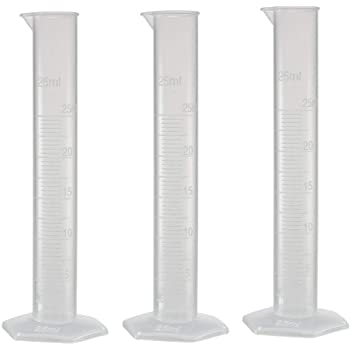
\includegraphics[width=5cm, height=5cm]{cylinders.jpg}
%DIF < %     \caption{Three graduated lab cylinders, corresponding to three
%DIF < %       eigenvectors. Prior eigenvalues not shown.}
%DIF < %     \label{fig:cylinder}
%DIF < % \end{figure}
}\DIFdelend \DIFaddbegin \DIFadd{for an illustration.
}\DIFaddend 




\DIFdelbegin \section{\DIFdel{Answer to Question \ref{q:why}: The cause of clusterization}}%DIFAUXCMD
\addtocounter{section}{-1}%DIFAUXCMD
%DIFDELCMD < \label{section:why}
%DIFDELCMD < %%%
\DIFdel{According to }\DIFdelend \DIFaddbegin \subsection{\DIFadd{Answer to Question \ref{q:why}}}\label{subsec:why}
\DIFadd{Building on }\DIFaddend Theorem \ref{thm:char}, \DIFaddbegin \DIFadd{we can now give a compelling
explanation to the measurement clusterization we observed for the
inverse problem of the heat equation, see Section
\ref{subsub:clusterization1} below. We also suggest a generic
explanation for clusterization, see Section \ref{subsub:clusterization2}.
}

\subsubsection{\DIFadd{Clusterization in the heat equation}}
\DIFadd{Consider $\fwd$ and $\prcov$ from }\emph{\DIFadd{the inverse problem of the
heat equation}}\DIFadd{. As before, we denote the eigenvalues of
$\fwd\prcov\fwd^*$ by $\lambda_j$. We input these eigenvalues into our
}\emph{\DIFadd{generic}} \DIFadd{model, and find a }\DIFaddend D-optimal \DIFdelbegin \DIFdel{designs aim to capture
a small subset of eigenvectors of the prior covariance, specifically
the $k$ eigenvectors with the highest prior variance. Our modelnaturally achieves this objective by not measuring eigenvectors $k+1$
and above, as proven in }\DIFdelend \DIFaddbegin \DIFadd{design $\opt$ for our
generic model using }\DIFaddend Theorem \ref{thm:char}. \DIFdelbegin \DIFdel{Translating this
understanding to spatial problems, we anticipate that }\DIFdelend \DIFaddbegin \DIFadd{In our generic model, the
measurements we take are best utilized in reducing uncertainty for the
first $k$ eigenvectors. So, }\DIFaddend a D-optimal design \DIFdelbegin \DIFdel{would favor measurement
locations where }\DIFdelend \DIFaddbegin \DIFadd{arising from our
}\emph{\DIFadd{generic model}} \DIFadd{completely avoids measuring eigenvectors $k+1$
and above.
}

\DIFadd{Of course, in a real life problem --- such as the inverse problem of
the 1D heat equation --- it is likely impossible to find measurement
locations for which all }\DIFaddend eigenvectors $k+1$ and above are
\DIFdelbegin \DIFdel{either close to zeroin value or possess small eigenvalues
in the prior spectrum, for some $k > 0$. To illustrate this
preference, Fig.~\ref{fig:why} depicts the scenario using the }\DIFdelend \DIFaddbegin \DIFadd{zero. However, if the eigenvalues of $\fwd\prcov\fwd^*$ decay quickly
(recall the square-exponential decay for eigenvalues of the }\DIFaddend 1D heat
equation \DIFdelbegin \DIFdel{with homogeneous Dirichlet boundary conditions (details
in the supplementary material)}\DIFdelend \DIFaddbegin \DIFadd{in eq.\eqref{eq:decay}), a D-optimal design will try to
balance measuring a small number (i.e.~$k$) of the leading
eigenvectors.
}

\DIFadd{The abovementioned balance is explored in
Fig.~\ref{fig:eigenvectors}. We allow $m=4$ measurements in $\Omega =
[0,1]$ and observe that D-optimal measurement locations are clustered
at $x_1 = 0.31$ and $x_2 = 0.69$. Upon close inspection of the scaled
eigenvectors of $\fwd \prcov \fwd^*$, we first observe that
eigenvectors $3$ and above have negligible prior amplitude. Since we
only have $m=4$ measurements at our disposal, we interpret these
results, following Theorem \ref{thm:char}, as implying we should only
care about measuring the first and second eigenvectors. Then, we note
the D-optimal $x_1,x_2$ present a compromise between the amplitude of
the first and second eigenvectors. For example, a measurement at
$x=0.5$ would have ignored the second eigenvector altogether, since
the second eigenvector is zero at $x=0.5$}\DIFaddend .
\DIFdelbegin \DIFdel{The plot showcases four eigenvectors }\DIFdelend \DIFaddbegin 

\DIFadd{Now we can understand measurement clusterization for the inverse
problem of the heat equation. A D-optimal design attempts to measure
the first $k$ eigenvectors of $\fwd \prcov \fwd^*$. But there may be
(spatial) limitations on where these $k$ eigenvectors have large
amplitude. For the inverse problem of the heat equation there are two
spatial locations that present a good compromise between the
amplitudes of the first and second eigenvectors}\DIFaddend , \DIFdelbegin \DIFdel{scaled according to their prior standard deviations. Since eigenvectors beyond the fourth have insignificant prior eigenvalues, we exclude them from consideration. Notably, we observe that
measurements are clustered near the zeros of
the third and fourth
eigenvectors, so we conclude that $k=2$. Clusterization arises because
there are only two
locations where the
third and fourth eigenvectorsapproach zero, while }\DIFdelend \DIFaddbegin \DIFadd{namely $x_1$ and
$x_2$ --- see Fig.~\ref{fig:eigenvectors}. We have $m=4$ measurements
at our disposal but only two spatial locations that are a good
compromise between }\DIFaddend the first and second \DIFdelbegin \DIFdel{eigenvectors exhibit
significantly non-zero values. Consequently,
when we allocate four
measurements to these two locations, they naturally cluster together, aligning with
}\DIFdelend \DIFaddbegin \DIFadd{scaled eigenvectors. Thus,
clusterization arises as a consequence of the pigeonhole principle.
}

\begin{figure}\label{fig:eigenvectors}
    \centering
    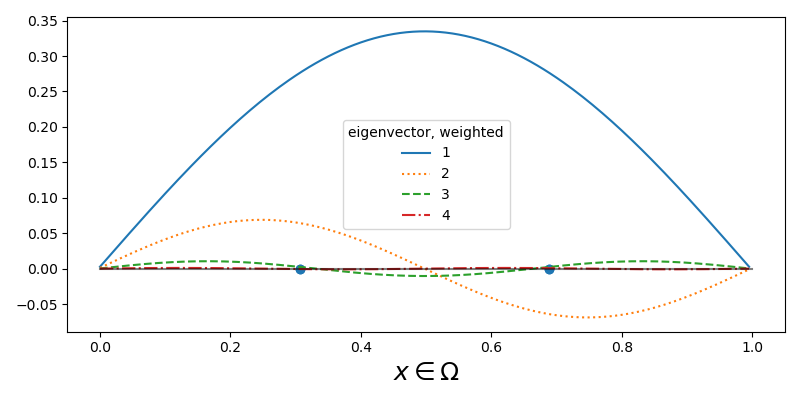
\includegraphics[width=\textwidth]{figs/eigenvectors_dst_scaled.png}
    \caption{\DIFaddFL{D-optimal measurement locations ($m=4$ measurements) and
      weighted eigenvectors for finding the initial condition of the
      1D heat equation. Measurement locations and weighted
      eigenvectors are plotted over the computational domain $\Omega =
      [0, 1]$ (x-axis). Measurement clusterization occurs
      approximately at $0.31$ and $0.69$. These two locations are a
      compromise between the magnitudes of the first and second
      eigenvectors, which are the eigenvectors that a D-optimal design
      aims to measure. Allocating $m=4$ measurements into two
      locations results in clusterization, according to the pigeonhole
      principle.}}
  \label{fig:why}
\end{figure}



\subsubsection{\DIFadd{Clusterization in our generic model}}\DIFadd{We can gain further insight to clusterization in our generic model,
from Carath\'eodory's Theorem and the concentration on the first $k$
eigenvectors of $\fwd \prcov \fwd^*$. We present a short discussion
adapting arguments presented in \mbox{%DIFAUXCMD
\cite[Chapter
  3]{silveyOptimalDesign1980} }\hskip0pt%DIFAUXCMD
and \mbox{%DIFAUXCMD
\cite[Section
  5.2.3]{pronzatoPazman2013}}\hskip0pt%DIFAUXCMD
.
}

\DIFadd{Consider $\opt$ a D-optimal design under our generic model.  As
instructed by Theorem \ref{thm:char}, we ignore all but the first $k$
eigenvectors of $\fwd \prcov \fwd$. Thus, we replace $\hilo$ with
$\hilo^{(k)}$ --- }\DIFaddend the \DIFdelbegin \DIFdel{pigeonhole principle}\DIFdelend \DIFaddbegin \DIFadd{$k$-dimensional subspace spanned by the first
$k$ eigenvectors of $\fwd^*\prcov\fwd$. Let
}\begin{equation*}
  \mathcal{M} := \conv \{\meas \meas^* : \meas\in \hilo^{(k)}, \|\meas\|=1\},
\end{equation*}
\DIFadd{where $\conv$ denotes the convex hull of a set. The set $\mathcal{M}$
contains only positive-definite operators on a $k$-dimensional vector
space. Hence $\mathcal{M}$ lives in a $k(k+1)/2$-dimensional vector
space. Since $\opt^*\opt = \sum_{i=1}^m \meas_i\meas_i^*$ for $\meas_i
\in \hilo^{(k)}$, it is easy to verify that $\frac{1}m \opt^*\opt \in
\mathcal{M}$.  Recall Carath\'eodory's Theorem:
}\begin{theorem}[Carath\'eodory]
  \DIFadd{Let $X \subseteq \mathbb{R}^n, X \neq \phi$ and denote $\conv (X)$
  the convex hull of $X$. For every $x \in \conv (X)$, $x$ is a convex
  combination of at most $n+1$ vectors in $X$}\DIFaddend .
\DIFaddbegin \end{theorem}
\DIFadd{Carath\'eodory's Theorem implies that there exist $\meas_i$ and
$\alpha_i$ such that
}\begin{equation*}
  \opt^*\opt = \sum_{i=1}^I \alpha_i \meas_i\meas_i^*,
\end{equation*}
\DIFadd{where $\|\meas\|=1, \sum\alpha_i = m, \alpha_i \geq 0$ and $I =
\frac{k(k+1)}{2} + 1$. We can thus write $\opt$ as:
}\DIFaddend 


\DIFdelbegin %DIFDELCMD < \bibliographystyle{ba}
%DIFDELCMD < \bibliography{../../lib.bib}
%DIFDELCMD < %%%
\DIFdelend \DIFaddbegin \[
\opt =
\left[
  \begin{array}{ccc}
    \horzbar & \sqrt{\alpha_i} \meas^*_1 & \horzbar \\
    \horzbar & \sqrt{\alpha_2} \meas_2^* & \horzbar \\
             & \vdots    &          \\
    \horzbar & \sqrt{\alpha_I} \meas_I^* & \horzbar \\
  \end{array}
\right].
\]
\DIFaddend 

\DIFaddbegin \DIFadd{Unfortunately, $\opt$ is not a valid design, since its rows do not
have unit norm. Still, the above representation of $\opt$ is useful:
If $m > \frac{k(k+1)}{2} + 1$, then $\alpha_i > 1$ for some $1\leq i
\leq I$.  Thus, we can view $\opt$ as a clustered design, since it
places weight $>1$ on a single measurement vector.
 }\section{\DIFadd{Numerical Experiments}}



\subsection{\DIFadd{Simulating Theorem \ref{thm:char}}}\label{subsec:lemma_sims}
\DIFadd{In the proof of Theorem \ref{thm:char} we utilize Lemma
\ref{lemma:free} to construct D-optimal designs. We implement this
construction with the goal of testing numerically how prevalent are
clustered designs. To this end, we would like to generate random prior
eigenvalues $\lambda_j$, fix $m$ and $k$, find a D-optimal
$\opt^*\opt$ and then utilize the construction of
Theorem~\ref{thm:char} and Lemma~\ref{lemma:free} to find $\opt$.
}


\DIFadd{To simplify things, we directly sample rank $\opt^*\opt$. We iterate
over the number of measurements $m \in \{4,\dots, 24\}$, and for every
$m$ we then iterate over $k:=\rank \obs^*\obs \in \{2,\dots,
m-1\}$. For each pair $m,k$ we repeat the following steps $N=5000$
times:
}\begin{enumerate}
\item \DIFadd{Generate random diagonal $D\in \mathbb{R}^{k\times k}$ with
  entries $\log (d_i) \sim \mathcal{N}(50,15)$ and normalize so that
  $\ttr D = m$. 
}\item \DIFadd{Conjugate $D$ by a random orthogonal matrix to form a positive
  semi-definite $M := UDU^t \in \mathbb{R}^{k\times k}$. This $M$
  represents $\opt^*\opt$.
}\item \DIFadd{Apply the construction of Lemma \ref{lemma:free} to calculate
  $A$ such that $AA^t = M$, where $A$ has unit norm columns. I.e.~find
  the optimal design $\opt$.
}\item \DIFadd{Since $A$ corresponds to $\opt$, its columns correspond to
  measurement vectors. We call $A$ "clustered" if $A$ has two or more
  identical columns (up to some numerical precision threshold).
}\end{enumerate}
\DIFadd{We then calculate the fraction of clustered designs of the simulations
we ran, for each pair $m,k$. Clusterization occurred at high rates
($>99.9\%$) whenever $m-k > 1$; see Fig.~\ref{fig:sim_AAt}. Hence, in
these simulations, clusterization is a generic property. However, when
$m-k = 1$, clusterization does not occur. We do not why this is so and
further investigation into this phenomenon is out of scope for the
current study.
}

\begin{figure}
    \centering
    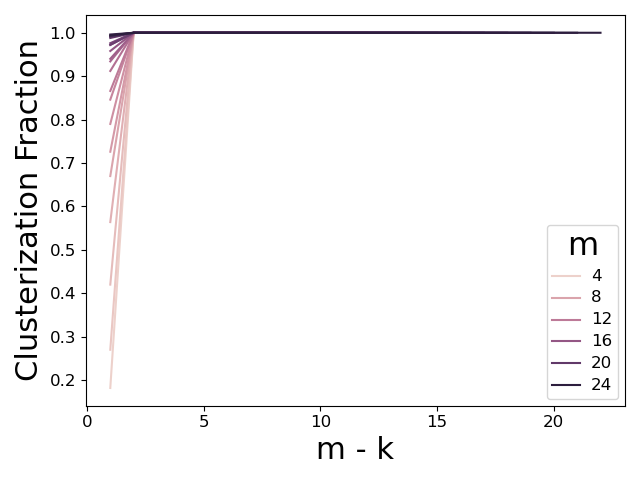
\includegraphics[height=0.5\textwidth]{figs/simulations.png}
    \caption{\DIFaddFL{Fraction of clustered $A$ for $AA^t = M$ and $M$
      generated randomly (see text and repository for details on
      generating $M$). It is evident that when $m-k \geq 2$ clusterization
      is ubiquitous, whereas for lower $m-k$ clusterization does not
      occur.}}
  \label{fig:sim_AAt}
\end{figure}

\DIFadd{Full results are located in the }\texttt{\DIFadd{simulations.csv}} \DIFadd{file within
the accompanying }\href{https://github.com/yairdaon/OED}{\DIFadd{repository}}\DIFadd{.
Code implementing the experiments described above is located in module
}\texttt{\DIFadd{zeros.py}} \DIFadd{of said repository. Runtime should be less than 30
minutes on any reasonably modern laptop (it took 12 minutes on the
author's laptop).
}


\subsection{\DIFadd{Correlated errors}}\label{subsec:corr_errors_sims}
\DIFadd{In order to verify the results of Section \ref{section:non_vanishing},
we run simulations of the inverse problem of the 1D heat equation with
nonvanishing model error \(\modcov = \prcov^2 \). Indeed, including
model correlation pushes measurements apart, see
Fig.~\ref{fig:corr_errors}. Code generating Fig.~\ref{fig:corr_errors}
is located in module }\texttt{\DIFadd{clusterization.py}} \DIFadd{in the accompanying
}\href{https://github.com/yairdaon/OED}{\DIFadd{repository}}\DIFadd{.
}

\begin{figure}
    \centering
    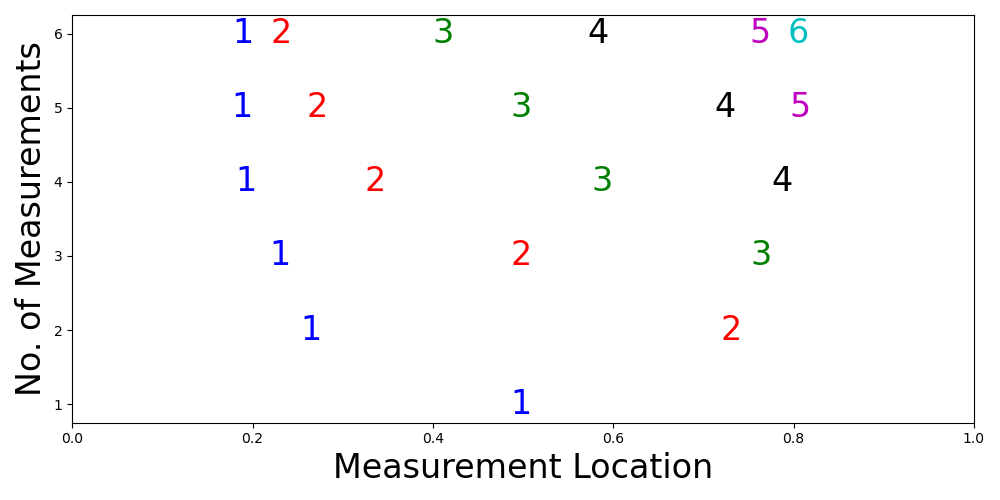
\includegraphics[height=0.5\textwidth]{figs/dst_modelError4.png}
    \caption{\DIFaddFL{Model correlation mitigates clusterization. We add a
      model correlation term to the error terms in the 1D heat
      equation inverse problem. Lo and behold, measurements are not
      close anymore and are pushed away thanks to the model error
      term.}}
  \label{fig:corr_errors}
\end{figure}



 


\DIFaddend \begin{acks}[Acknowledgments]
  This study is a result of research I started during my PhD studies
under the instruction of Prof.\DIFaddbegin \DIFadd{~}\DIFaddend Georg Stadler at the Courant Institute
of Mathematical Sciences. I would like to thank him for his great
mentorship, attention to details and kindness. I would also like to
thank Christian Remling, who helped me find a proof for Lemma
\ref{lemma:free} in
\href{https://mathoverflow.net/questions/280168/redistribute-diagonal-entries-of-a-matrix/280203#280203c}{Mathoverflow}.
\DIFaddbegin \DIFadd{Last, but certainly not least, I would like to thank the three
referees, associate editor and editor in chief for providing detailed
and insightful reviewes that have made this manuscript a whole lot
better.
   }\DIFaddend 

  This research was supported in part by an appointment with the
National Science Foundation (NSF) Mathematical Sciences Graduate
Internship (MSGI) Program sponsored by the NSF Division of
Mathematical Sciences. This program is administered by the Oak Ridge
Institute for Science and Education (ORISE) through an interagency
agreement between the U.S. Department of Energy (DOE) and NSF. ORISE
is managed for DOE by ORAU. All opinions expressed in this paper are
the author's and do not necessarily reflect the policies and views of
NSF, ORAU/ORISE, or DOE.
 %DIF <  This work was also supported by The Raymond and Beverly Sackler
%DIF <  Post-Doctoral Scholarship.
\end{acks}
\DIFaddbegin 

\bibliographystyle{ba}
\bibliography{../../lib.bib}
\DIFaddend 


\end{document}
